\documentclass{article}

\usepackage[margin = 3cm]{geometry}
\usepackage[table]{xcolor}
\usepackage{graphicx}
\usepackage{hyperref}
\usepackage{listings}
\usepackage{color}
\usepackage{lipsum}
\usepackage[margin=1cm]{caption}

\definecolor{codegray}{gray}{0.9}
\definecolor{mygreen}{rgb}{0,0.6,0}
\definecolor{mygray}{rgb}{0.5,0.5,0.5}
\definecolor{mymauve}{rgb}{0.58,0,0.82}
\captionsetup{format=hang}
\pagestyle{headings}
\pagecolor{white}

\lstset{ 
  backgroundcolor=\color{white},   % choose the background color; you must add \usepackage{color} or \usepackage{xcolor}; should come as last argument
  basicstyle=\footnotesize,        % the size of the fonts that are used for the code
  breakatwhitespace=false,         % sets if automatic breaks should only happen at whitespace
  breaklines=true,                 % sets automatic line breaking
  captionpos=b,                    % sets the caption-position to bottom
  commentstyle=\color{mygreen},    % comment style
  deletekeywords={...},            % if you want to delete keywords from the given language
  escapeinside={\%*}{*)},          % if you want to add LaTeX within your code
  extendedchars=true,              % lets you use non-ASCII characters; for 8-bits encodings only, does not work with UTF-8
  firstnumber=1000,                % start line enumeration with line 1000
  frame=single,	                   % adds a frame around the code
  keepspaces=true,                 % keeps spaces in text, useful for keeping indentation of code (possibly needs columns=flexible)
  keywordstyle=\color{blue},       % keyword style
  language=Octave,                 % the language of the code
  morekeywords={*,...},            % if you want to add more keywords to the set
  numbers=left,                    % where to put the line-numbers; possible values are (none, left, right)
  numbersep=5pt,                   % how far the line-numbers are from the code
  numberstyle=\tiny\color{mygray}, % the style that is used for the line-numbers
  rulecolor=\color{black},         % if not set, the frame-color may be changed on line-breaks within not-black text (e.g. comments (green here))
  showspaces=false,                % show spaces everywhere adding particular underscores; it overrides 'showstringspaces'
  showstringspaces=false,          % underline spaces within strings only
  showtabs=false,                  % show tabs within strings adding particular underscores
  stepnumber=2,                    % the step between two line-numbers. If it's 1, each line will be numbered
  stringstyle=\color{mymauve},     % string literal style
  tabsize=2,	                   % sets default tabsize to 2 spaces
  title=\lstname                   % show the filename of files included with \lstinputlisting; also try caption instead of title
}

\newcommand{\type}[1]{\smash{\colorbox{codegray}{\texttt{#1}}}}
\graphicspath{ {./Images/} }

\date{\today}

\begin{document}
\begin{titlepage}

    \centering
    
    \hspace{2cm}
\includegraphics[scale=1.0]{uulogo.png}

	\vspace{1cm}
	{\Large \textsc{Computing Science Master Thesis}\par}
	\vspace{1.0cm}
	{\huge\bfseries Polymorphic Variant Types in Data-Parallel Languages \par}
	\vspace{1.5cm}

    \begin{abstract}
        Data-parallelism uses the uniformity between multiple data elements to accelerate the process of operating on large collections of data.
        Variant types constrain the ability to operate uniformly, which therefore limit data-parallelism opportunities in the general case.
        In the situations where non-uniformity is inherit to the algorithm low-level optimizations are used to mitigate the heterogeneity.
        In this paper a higher abstraction level variant type is explored which can capture the required low-level control to be able to represent these optimizations in data-parallel languages.
        A polymorphic variant type is used to represent variability on the type-level, which is used by data structures to adapt to the identity of the variant type.
        Type-level programming is used to derive memory efficient representation for user-defined datatypes.
        (De)construction of variant types is automated through datatype-generic programming, which means custom memory representations can be provided seamlessly.
        It results in a fully modular variant type that can exercise low-level control while preserving the type identity of variant.
        An implementation is provided in the data-parallel language {\it Accelerate}, which demonstrates the viability of variant types in a data-parallel context.

    \end{abstract}

	\vfill

    %\raggedright
    {\Large Luuk de Graaf, 66577830. \par}

    \vspace{0.5cm}
    {\normalsize First supervisor   : Gabriele Keller \par}
    {\normalsize Second supervisor  : Wouter Swierstra \par}

\end{titlepage}

\newpage

\tableofcontents

\newpage

\section{Introduction}

Array languages can operate on a higher abstraction level and implicitly execute instructions in parallel on multiple elements. 
A data-parallel \type{map} and \type{fold} function is sufficient to cover a wide range of high-performance applications.
A naive intersection algorithm for a raytracer can be defined incredibly concisely compared to a handwritten c++ implementation.

\begin{verbatim}
    nearest :: Ray -> [Triangle] -> Float
    nearest ray = fold min 1e30f . map (intersect ray)

    float nearest(Ray ray, Triangle tri)
    {
        float4 minimum4 = float4(1e30f, 1e30f, 1e30f, 1e30f);
        for (int i = 0; i < objects.Length / 4; i += 4)
        {
            float4 dist4 = intersect(ray, tri[i], tri[i + 1], tri[i + 2], tri[i + 3]);
            minimum4 = min(minimum4, dist4);
        }
        float minimum = min(min(minimum4.x, minimum4.y), min(minimum4.z, minimum4.w))
        for (int i = 0; i < objects.Length % 4; i++)
        {
            float distance = intersect(ray, tri[objects.Length + i]);
            minimum = min(minimum, distance);
        }
        return minimum;
    }
\end{verbatim}

A consideration for working on a higher-abstraction level is the lack of low-level control, which can be crucial in performance sensitive cases.
Sometimes it is easy to incorporate optimizations, with the example of the \type{nearest} function using the sentinel value \type{1e30f} to avoid returning an explicit failure state\footnote{A tag would require branching on the result, which hinders data-parallelism in the general case.}.
In other cases this is significantly harder, such as low-level optimizations around memory representation and cache efficiency.
This is made apparent when attempting to extend the intersection function to operate on other primitives, such as spheres.
The path of least resistance is to create a datatype that can either be a triangle or a sphere.

\begin{verbatim}
    data Primitive = Triangle ... | Sphere ...

    nearest :: Ray -> [Primitive] -> Float
    nearest ray = fold min 1e30f . map (intersect ray)
\end{verbatim}

Such datatype can also be used to return the specific primitive that was hit. 
In the general case\footnote{When the branching does not diverge within a warp, which is the case when the array is sorted, a GPU will have very little overhead.} this will unfortunately hinder data-parallelism as it requires branching on the identity of the object.
A solution is to handle primitives as standalone types with their own respective collection, which can be achieved nicely with an uniform interface.

\begin{verbatim}
    class Primitive a where
        intersect :: Ray -> a -> Float

    nearest :: (Primitive a) => Ray -> [[a]] -> Float
    nearest ray = fold min 1e30f . fold (map (intersect ray)) 1e30
\end{verbatim}

\newpage

While we improved the possibility for data-parallelism, we still need to maintain the \type{Primitive} datatype when we want to explicitly return which primitive was hit.
To improve our naive O(n) implementation we can use an acceleration structure to eliminate primitives prematurely based on their spatial properties.
This means intersections will be performed in smaller batches, to be able to exit early, which reduces the opportunities for data-parallelism.
From a performance standpoint it might be preferable to separate the primitives on a batch-level, requiring even another datatype.
Maintaining the architecture around all these different constructs is ergonomically not viable and caused by our attempt to achieve low-level control.  
The intent of all approaches remains interchangeable, which is to operate on a collection with multiple variants of a type.
A type-safe and generic implementation is often not possible, as datatypes and interfaces must be defined at compile time.
It is also not feasible to manually define mappings between all these different representations.

\begin{verbatim}
    // value-level tagged union with a closed system 
    data Primitive = Triangle ... | Sphere ...

    // type-level interface with an open system
    class Primitive a where
        intersect :: Ray -> a -> Float
\end{verbatim}

The inability to abstract over both value-level variant types and type-level variant types prevent a generic higher level abstraction from taking form.
Unifying these concepts would allow a collection of primitives to be fully agnostic to the underlying representation.
Within this paper we propose a way to ergonomically switch between representations for collections of variant types.
Type-safety is preserved by elevating the concept of a mutually exclusive datatype to the type-level, which is achieved through type-level and datatype-generic programming.
An implementation can exist without it being natively supported as construct in the implementation language.
This can be utilized by libraries, frameworks and embedded domain-specific languages that exist in languages that facilitate type-level programming and datatype-generic programming, like Haskell.

\begin{verbatim}
    image: explain type-level variant type


\end{verbatim}

Such implementation also gives the opportunity to give low-level control on both the memory representation and the (de)-construction of variant types. 
Control over the memory representation is invaluable for adapting to cache behavior without having to change the architecture around it.
Manual control over the (de)-construction would also prevent the need for the explicit sentinel value in our intersection algorithm.
The failure state \type{Nothing} can be used, which is internally represented as \type{1e30f}.
The \type{min} function uses the value directly while other functions must pattern match on the value \type{1e30f}.
Within the context of raytracing this other function might spawn an extension ray that simulates the ray bouncing of a surface.
Pattern matching on the \type{1e30f} value will limit data-parallelism for all subsequent extension rays.
A solution can be to unconditionally execute like with the \type{min} function or eliminate all rays that failed for each iterative step. 
The latter can now be represented as an internal reorganization in the proposed implementation, as it does not change the identity of the collection but merely the layout and thus no architectural changes are required.
To summarize, the goal of this paper is to improve the experience of operating on a collection of multiple variants.
The primary question pertains to how variant types can be implemented with adaptability to low-level optimizations within a data-parallel context.
The contribution of this paper includes:

\begin{itemize}
    \item An extendable deduplication algorithm for variant types. 
    \item Automatic derivation of an isomorphic mapping between any two datatypes. 
    \item A collection of multiple variants that is completely agnostic to its internal representation.
\end{itemize}

\newpage

\subsection{Related Work}

Initial objective was establishing a computational efficient representations for non-uniform data in data-parallel applications.
This induced the need for a flexible and type-safe interface, which has been achieved through type-level and datatype generic programming.
Relevance is established by an implementation in the data-parallel language Accelerate, which is deeply embedded within Haskell.

\paragraph{Performance}

The memory representation of a datatype is often based on the functionality they perform within a language.
In data-parallel applications primitive types are distributed over multiple arrays to facilitate vectorization.
It is not apparent what the representation of a tagged union should be, as they inherently break vectorization in most cases. 
The functional data-parallel languages Accelerate\cite{accelerate-sum-types} and Futhark\cite{futhark-sum-types} implicitly distribute primitive types in composite datatypes over multiple arrays.
Both implementations have limited deduplication capabilities, but research has been done to integrate a memory efficient tagged union in Accelerate\cite{accelerate-sum-types}.
Game-engines, which deal with many clusters of data, have a fundamentally different approach as they have widely adopted the Entity-Component-System (ECS) pattern. 
Many implementations incite a collective re-organization of the internal representation when a variant change occurs at runtime.
A type-safe and performant implementation is notably hard due to having to statically resolve all interactions between the representations, which means meta-programming and untyped code are extremely prevalent. 

\paragraph{Interface}

Functional languages handle tagged unions safely through Algebraic Data Types (ADTs), where sum types categorize ADTs with multiple variants.
Constructors can be local to an unique ADT (nominally typed) or exist as independent types (structurally typed).
Deconstructing is done by pattern matching, where functions natively branch on the current active variant.
In Haskell sum types are nominally typed, which means variants are not standalone types and cannot exist safely outside the ADT.
Structural sum types are often called extensible or open sum types, as they do not have to be explicitly declared before use.
In OCaml these are natively supported as polymorphic variants, while Futhark is completely structurally typed and refers to them as sum types.
Deriving an efficient internal representation for a user-defined datatype can be done statically by type-indexing types\cite{associated-types}, which are called {\it traits} in c++.
Some libraries also create a low-level abstractions which allows for custom memory representations \cite{llama} or employ meta-programming to be flexible in the memory representation.
Datatype-generic functions, which parametrize on the structure of a datatype, can be used to create mappings between these computed representations.
Both concepts are used in highly generic libraries for a wide-range of applications\cite{generic-programming}. 

\paragraph{Implementation}

Variant types are rare in array languages, likely due to the infrequency of non-uniform data in data-parallel applications and the required low-level control in the instances they are needed.
In functional languages such as Accelerate and Futhark they arguably only exist to complete the ADT archetype.
Some implementation details are therefore primarily centered around these two languages.
Accelerate is a data-parallel array language deeply embedded within Haskell, where sum types are currently represented as a non-compact tagged union.
Research has been done on a compact tagged union representation for parallel arrays, which has been named a {\it Recursive Tagged Union}\cite{accelerate-sum-types}.
The representation uses a unified tag for nested sum types, which optimizes memory usage at the cost of tag (de-)construction but has not yet been implemented. 
This paper fundamentally distinct itself by looking beyond the sum type and implementing an extendable and modular interface, rather than a single concrete layout. 
Futhark is a functional structurally typed data-parallel array language, where only identical primitive types are deduplicated.
The research pertains primarily on including structural sum types to the Futhark compiler\cite{futhark-sum-types}.

\newpage

\section{Performance}

It is fundamental to understand performance implications when creating a higher level abstraction in a performance critical environment.
There are many components that can influence the performance of a program.
This grows the importance of being able to identify {\it bottlenecks} but also understanding the underlying technological performance considerations.
Within the first section fundamental optimizations related to the interaction between data and hardware are introduced.
This is used to identify architecture agnostic performance considerations for operations on collections of data in the second section.
In the third section this information is used to enumerate efficient data structures for multiple variants of a type.

\subsection{Optimizations}

In the early days of computing, memory was seen as a way to store data indefinitely.
As computational power of processors increased, the importance of main memory increased.
Main memory is dependant on the advancements of random-access-memory (RAM), which stagnated due to both cost and physical limitations\cite{memory}. 
This put pressure on the software side to adapt to hardware components for optimizations, rather than merely the computational complexity of algorithms.
One of these hardware optimizations is cache storage, which accelerates memory accesses of predetermined data.
The chosen data is decided based on a cache replacement policy, often based on a temporal property. 
The cache operates independently of the operating system\cite{memory}, and no direct control can be exercised.

\begin{figure}[ht]
    \centering
    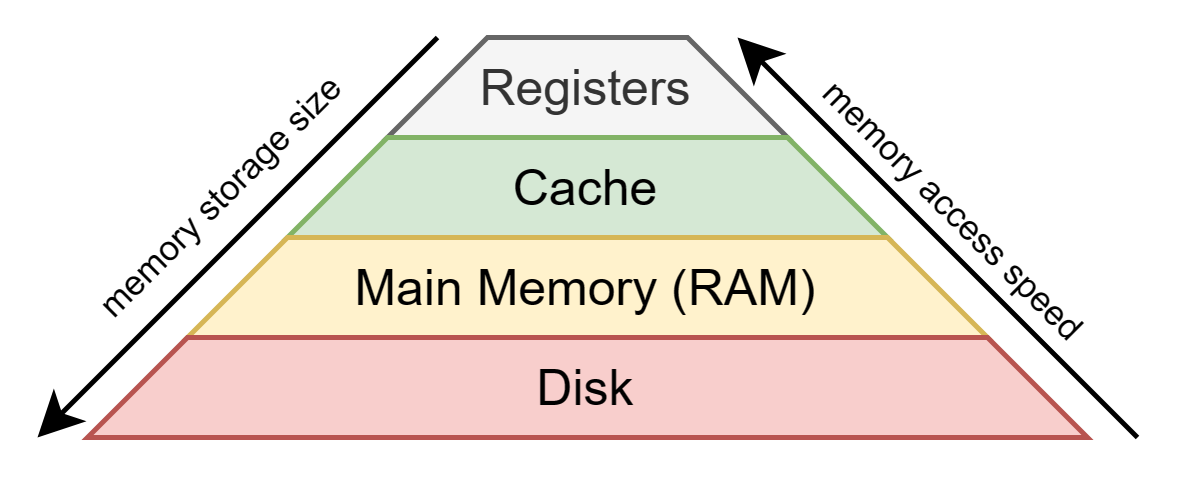
\includegraphics[scale=0.2]{memoryhierarchy}
    \caption
    {
        An abstract view of a computer memory hierarchy. 
        Each layer can be subdivided even further, depending on the type of hardware. 
        The difference between both the memory access time and memory storage size for each layer can be several order-of-magnitudes.
        As example: data in a register effectively takes 0 instruction cycles, while data from disk might take several million instruction cycles to arrive.  
    }
\end{figure}
\paragraph{Instructions}

Interfacing with processors is done through computer instructions.
Fetching of an instruction is a memory operation in itself, as it retrieves the instruction at the target of the program counter.
Instructions operate on registers, which have distinct sizes depending on the architecture and their respective function.
There are many instruction set architectures (ISA) and devices that utilize only a specific instruction set.
An intermediate representation (IR), such as the LLVM IR\cite{LLVM}, can be used to create a single interface for multiple instruction sets\cite{intermediate-representation}.
Hardware design sometimes allows for specialized instructions\footnote{Note that this is separate from a {\it complex instruction}, which concerns a compact {\it representation} of several instructions. }, which are faster than their semantically equivalent instruction(s).
Examples include sacrificing accuracy for performance (floating-point), combining a sequence of instructions (arithmetic) or by parallel execution on multiple data elements (SIMD).
SIMD instructions in particular are often very performant, as several steps within the execution pipeline can be parallelized.
The process of parallelization of multiple instructions is called {\it vectorization}.
Using these architecture dependant instructions directly can be achieved through compiler intrinsics.

\begin{figure}[ht]
    \centering
    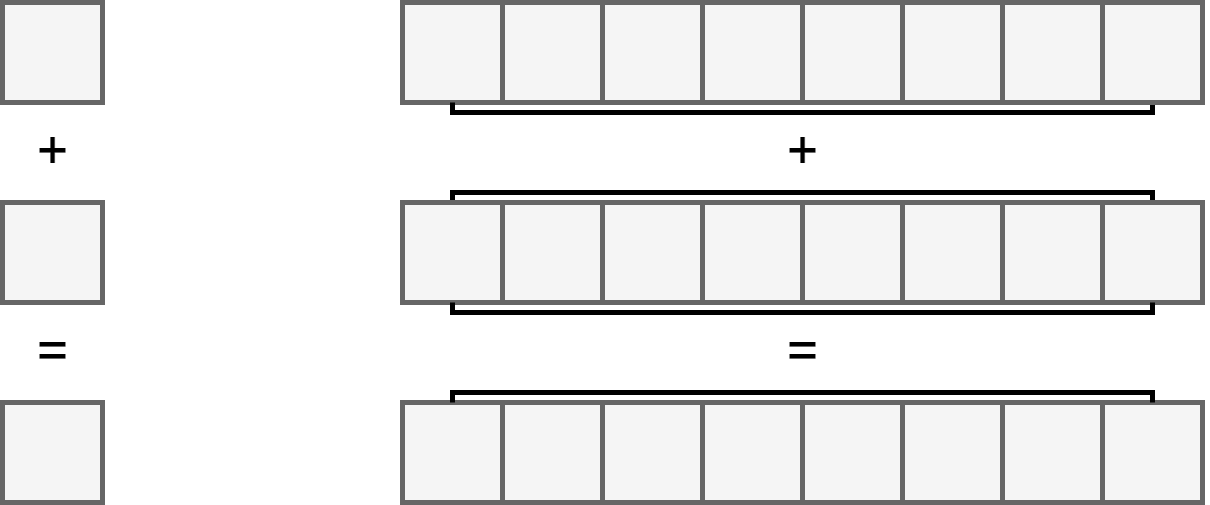
\includegraphics[scale=0.2]{vectorization}
    \caption
    {
        A scalar addition instruction is converted to the equivalent single instruction multiple data (SIMD) instruction, where each grey square denotes a single data component.
        Vectorization requires the data to be contiguous in memory and effectively performs the work of several scalar operations within a single instruction.  
    }
\end{figure}

\newpage

\paragraph{Register Pressure} 

Registers can be considered the fastest available memory, as the data is ready to be used by an instruction.
Within the context of registers this data is commonly referred to as a variable.
Variables existing within registers before execution is a prerequisite for reasonable performance.
The scheduling problem of ensuring all variables exist in registers before execution is to be considered a NP-complete problem\cite{register-allocation}.
Programming languages with any form of abstraction generally delegate this process to the compiler.
It simplifies a lot of complexity, as only which data is being used by what instruction is relevant for the programmer.
In some cases there are too many live variables for the available registers, which can {\it spill} the variable.
This requires a variable to be stored outside registers, in a slower form of memory, and incites a delay when attempting to use the data.
It can be prevented by either reducing the time variables are live, reordering the sequence of instructions or diversifying the execution units.  

\paragraph{Memory Access Time}

Semantically random-access-memory (RAM) implies that memory operations take around the same amount of time, independent of the physical storage location.
In practice this does not hold for several reasons.

\begin{itemize}
    \item [SRAM/DRAM]
    On a modern system there often exist several different types of RAM, mostly driven by cost differences.
    The main forms of RAM are static RAM (SRAM) and dynamic RAM (DRAM).
    SRAM uses six transistors to represent a single bit, while DRAM only uses one transistor with a single capacitor. 
    A capacitor loses electrons over time which means data has to be refreshed repeatedly to preserve its data.
    A refresh requires both read and write operations, which interferes with other memory operations.
    This makes DRAM inconsistent and on average significantly slower but much cheaper to produce due to requiring less transistors.\cite{memory}

    \item [Propagation]
    Data is transferred by using electrical charges through semi-conductors.
    This creates a physical limitation dictated by physical distance and temperature.
    This is called propagation delay and a hard limitation to the rate at which components can operate on.
    SRAM is often located physically closer to the execution units to utilize the faster memory access more effectively.
 
    \item [DMA]
    A processing unit needs to forward the requested data to the targeted location, which takes up processing time.
    Direct-memory-access (DMA) is an interface for hardware components and allows memory operations to be more organized.
    This allows for large scale memory operations to be performed efficiently and independently of the main processor.
    It requires use of several buses which means some processors must idle at seemingly random periods of time.
    In essence it means that other hardware components can influence the memory access time.
 
\end{itemize}

\newpage

\paragraph{Caching}

Due to discussed hardware related discrepancies in memory access time, it can be beneficial to organize data according to the memory access time.
The simplest way to achieve this is by caching data, that is storing a {\it copy} of the data in a faster accessible medium.
A cache generally consists of SRAM and resides close to the processor, which allows memory accesses to be order-of-magnitudes faster than a main memory access\cite{memory}.
When data already exist in the cache it is referred to as a cache hit, otherwise a cache miss has occurred.
Deciding which data is cached and for how long is a cache replacement policy, utilizing both recency and frequency.
Adapting to policies simplifies both the scheduling and minimizes the potential cache misses that can occur in the worst case scenario.

\begin{figure}[ht]
\begin{minipage}{.65\textwidth}
Caching of data can be done after the data has already been retrieved, which means a delay already has occurred.
This can be avoided by requesting data in advance and storing the data in a cache prematurely, so called cache {\it prefetching}.
It can be accomplished by analyzing future instructions (hardware) or using instructions that {\it hint} at the future use of a piece of data (software)\cite{cache-prefetching}.
Prefetching is harder when there are multiple execution paths possible, as both the data and the next instructions will be uncertain.
Speculatively executing the uncertain instructions can be performant if the overhead of redundant work remains small enough.
Rather than executing unconditionally, some processors execute the most likely to happen branch based on some parameters (branch prediction)\cite{instruction-level-parallelism}.
\end{minipage}%
\begin{minipage}{.35\textwidth}
    \centering
    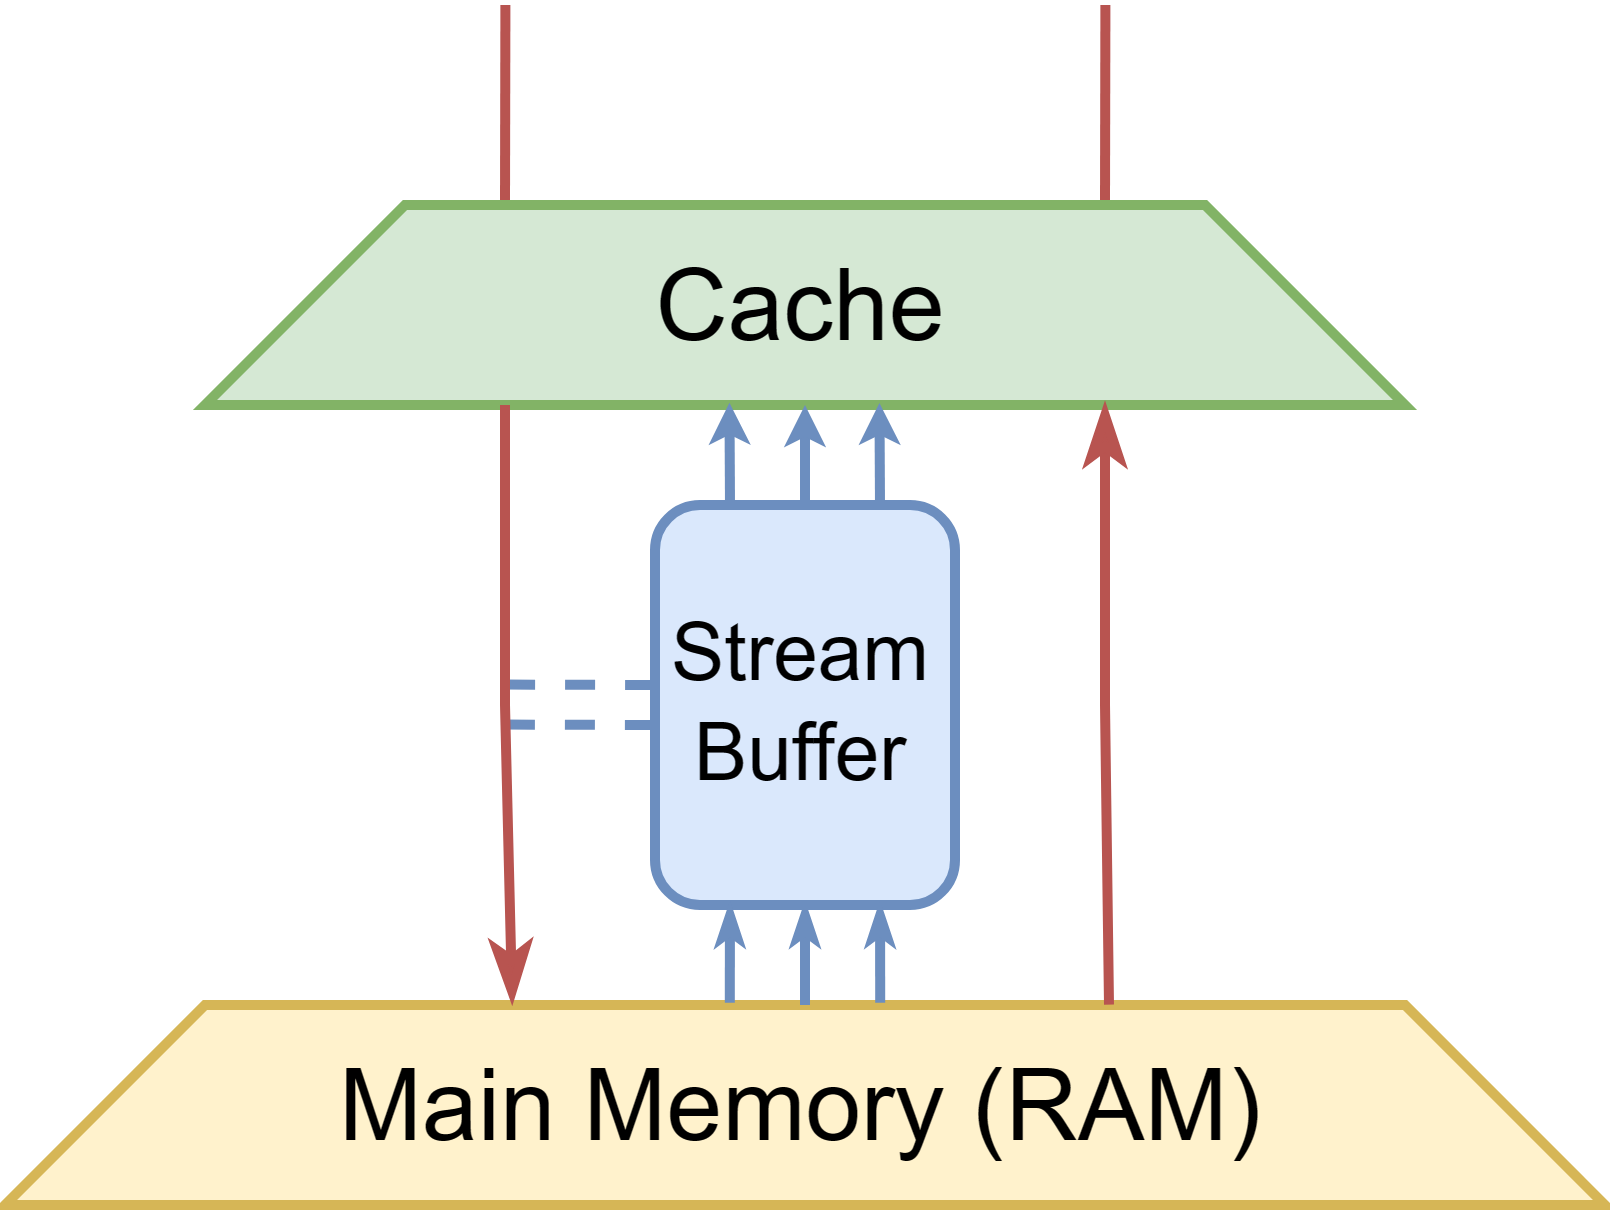
\includegraphics[scale=0.08]{cache (2).png}
    \captionsetup{margin=0.5cm}
    \captionsetup{format=plain}
    \caption{Stream buffer that prefetches data into the cache based on cache misses.}
\end{minipage}
\end{figure}
\vspace{-1.5em}
\paragraph{Parallelism}
Instruction-level parallelism is the parallel execution of multiple instructions\cite{instruction-level-parallelism}.
It can be done by dividing an instruction into several steps and outsourcing each step to a distinct processor unit (instruction pipelining).
Shuffling the order of instructions might allow more units to work in parallel from each other (out-of-order execution).
This can be extended by outsourcing instructions to different units of the same type, such as execution units (superscalar execution).
An abstraction-level higher is data-level parallelism, which executes a single instruction on multiple data elements such as the previously discussed SIMD instructions.
Specialized processors sometimes either fully pipeline the data (vector processing) or allow for some form of autonomy (multithreading). 
Both share instruction fetching and decoding, but threads have their own program counter which allows for an independent sequence of instructions.
Execution of threads can be done concurrently, which can be useful to hide latencies (context-switching).
In parallel is also possible with multi-core processors, which have several processors units (cores) that can support multiple threads at the same time.
Cores are often not independent processors and might share several components with other cores, such as caches\cite{thread-level-parallelism}.

\begin{figure}[ht]
    \centering
    \begin{minipage}{.5\textwidth}
        \centering
        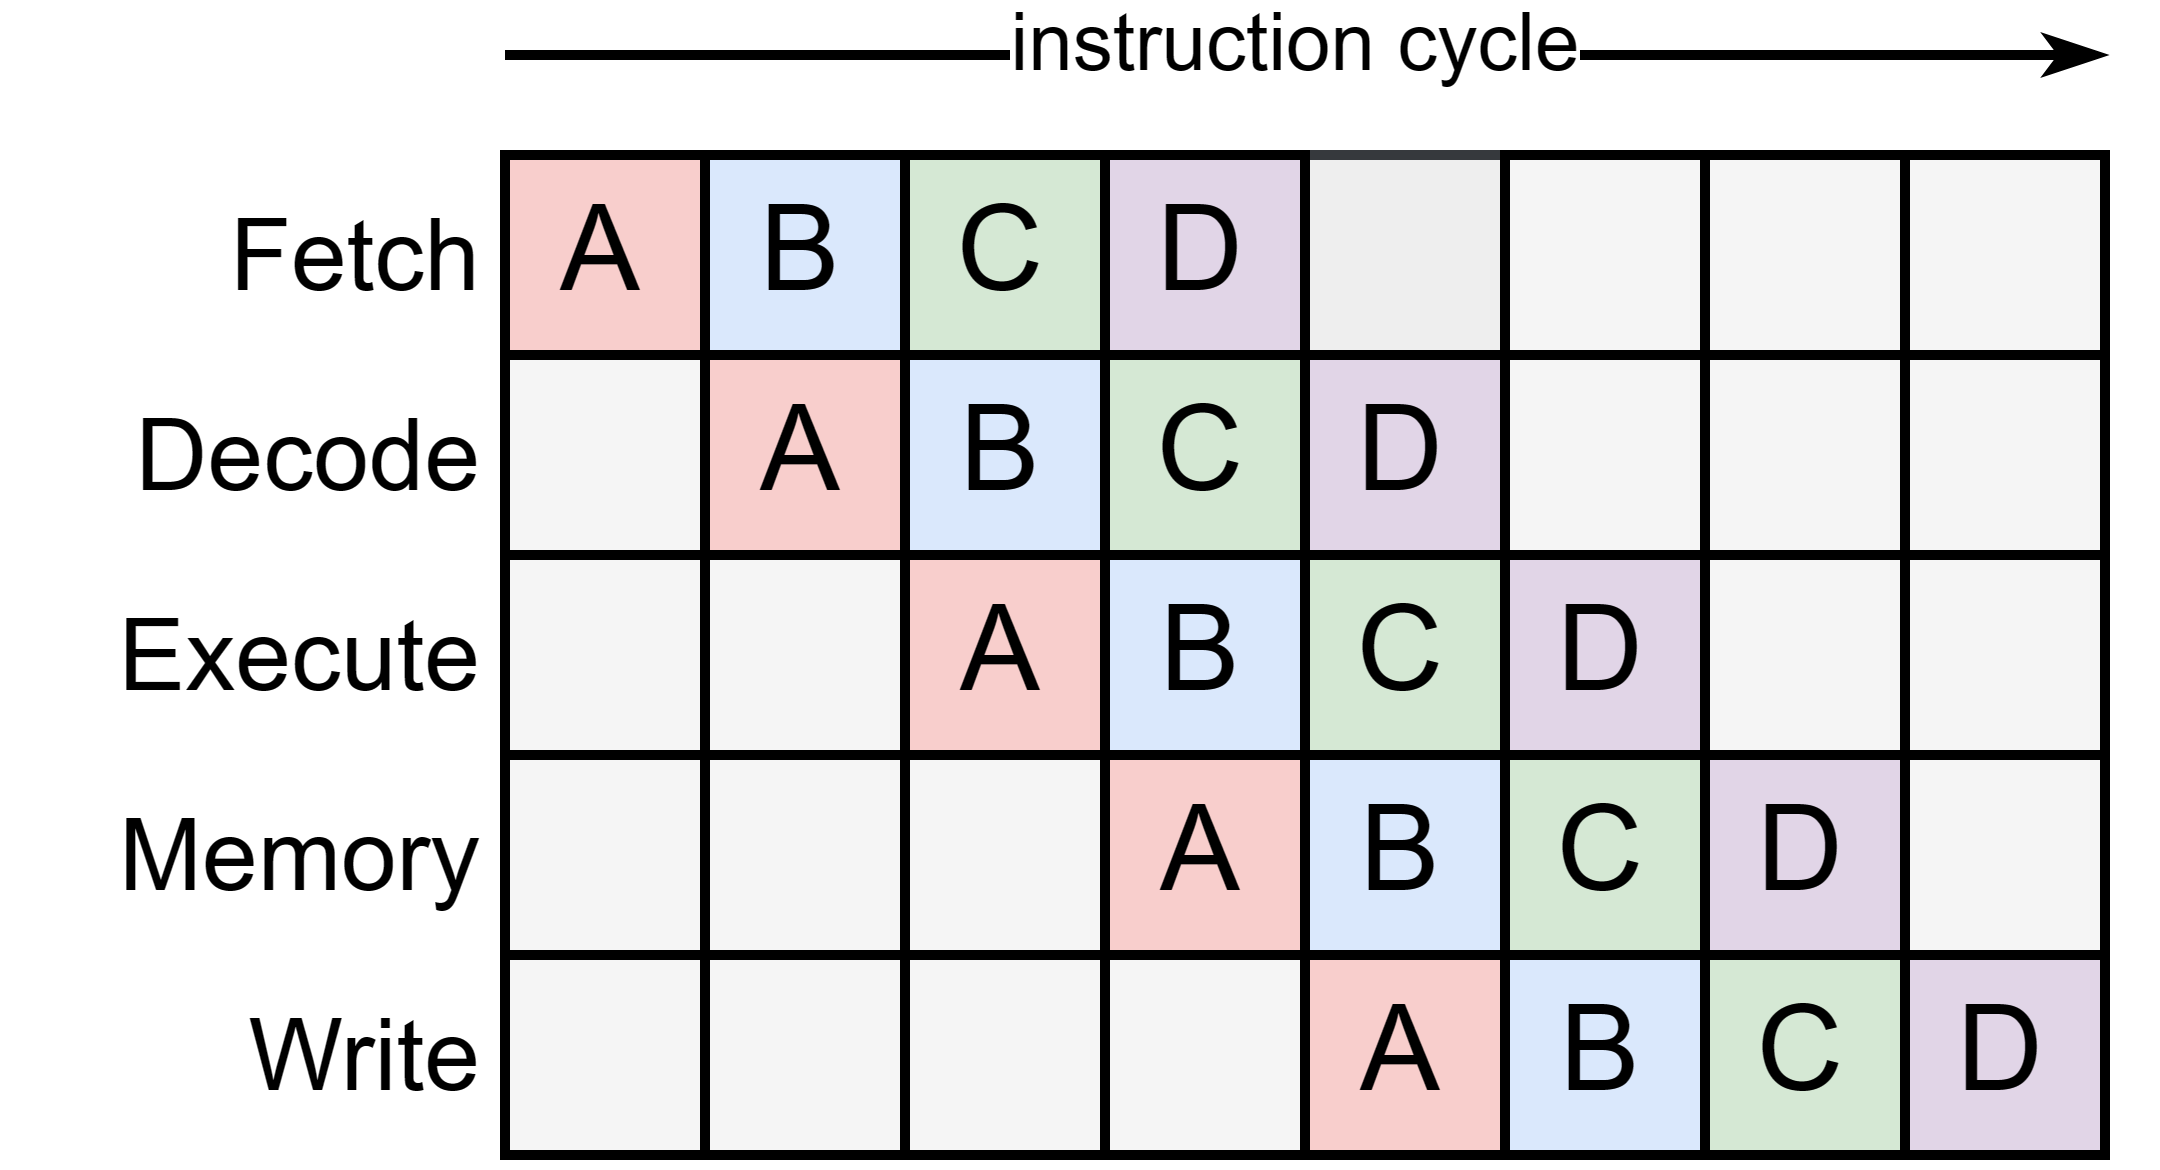
\includegraphics[scale=0.09]{instructionpipeline.png}
        \captionsetup{margin=0.2cm}
        \caption
        { 
            Multiple phases allows a processor to hypothetically execute the [A, B, C, D] instructions in 8 cycles.
            This is significantly faster in comparison to the 20 cycles it would require in a single lane.
        }
    \end{minipage}%
    \begin{minipage}{.5\textwidth}
        \centering
        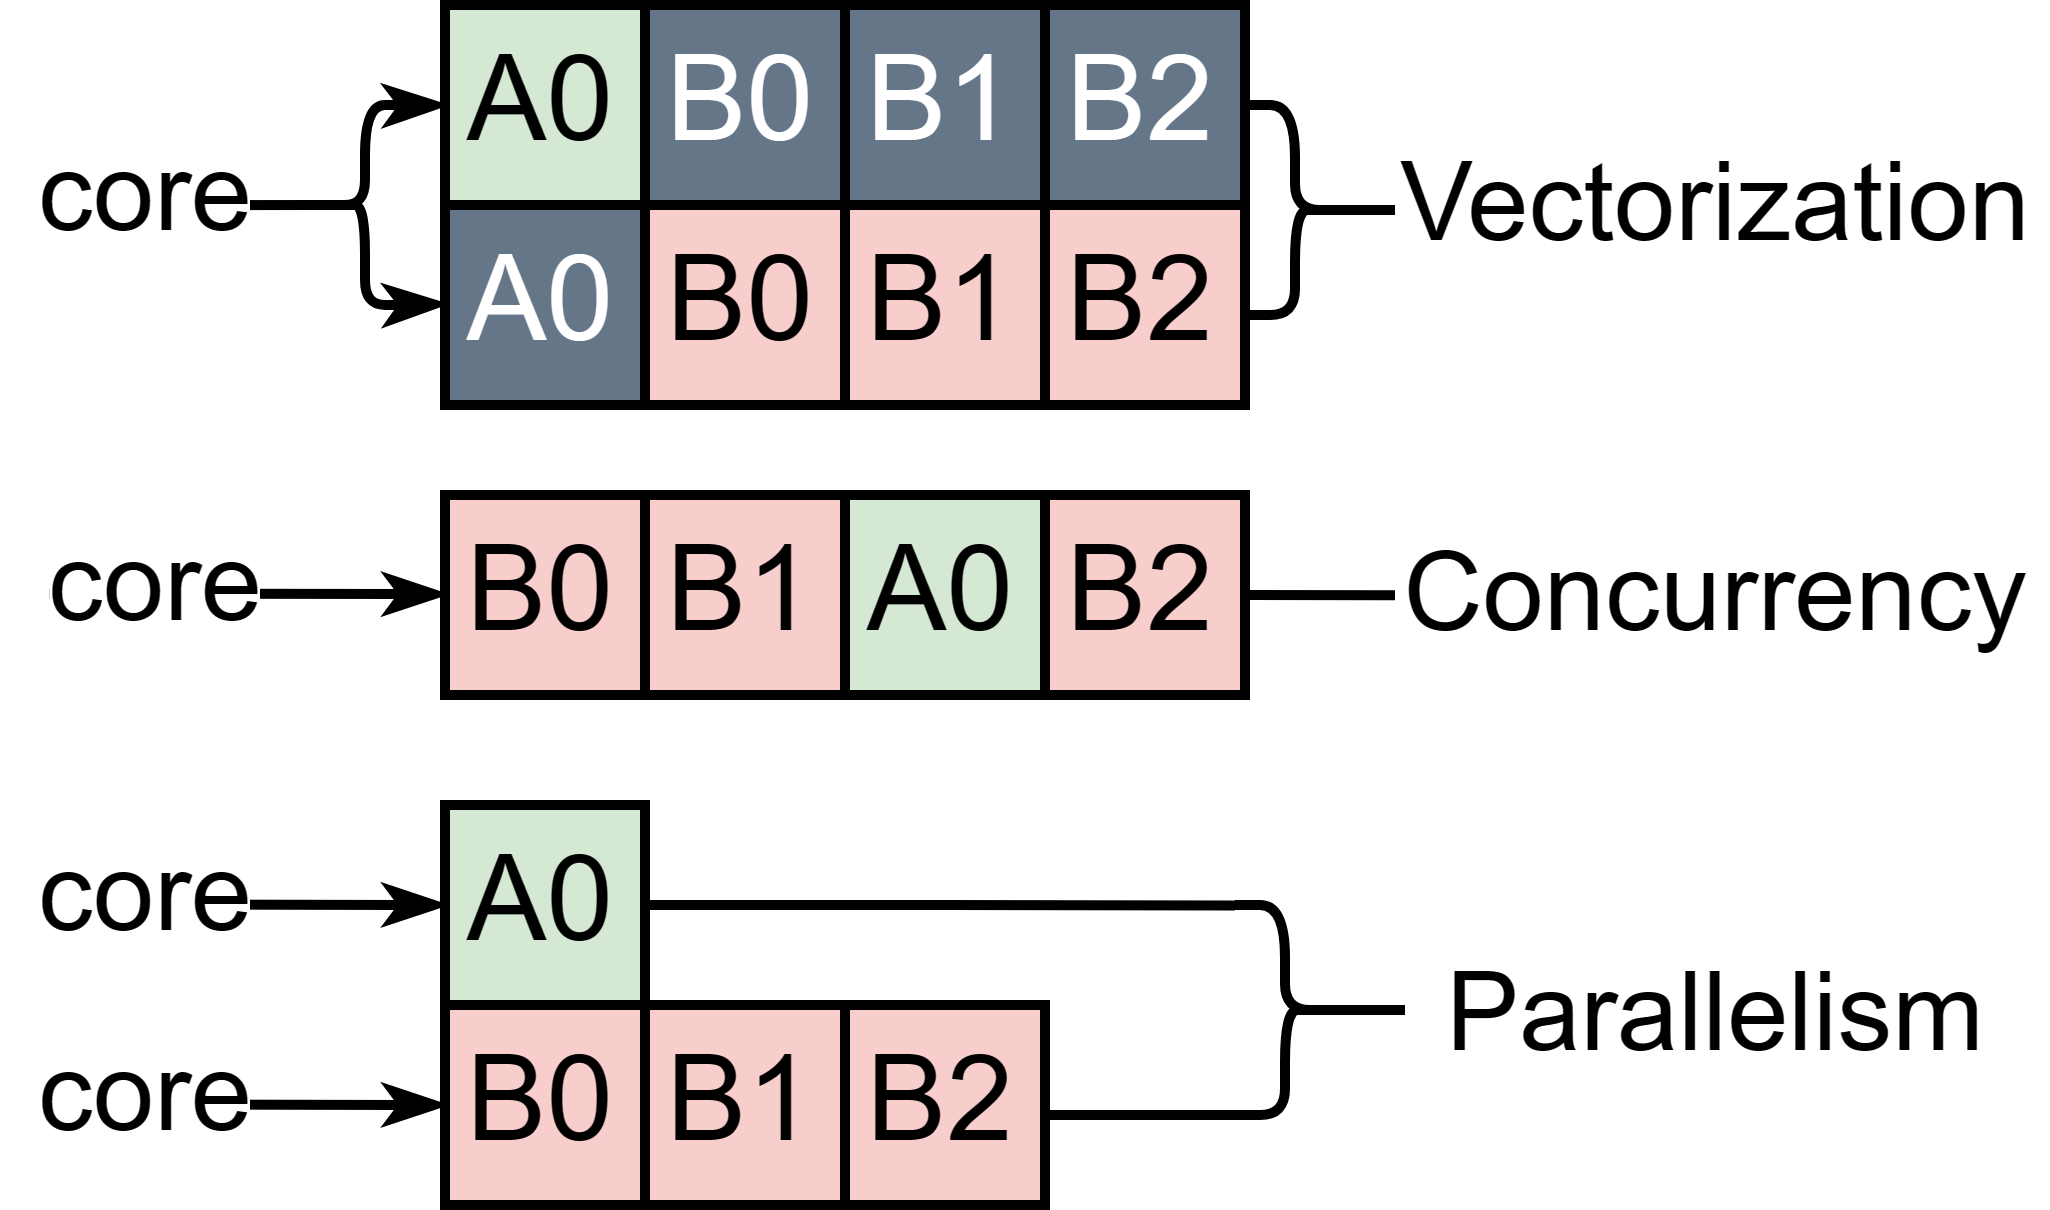
\includegraphics[scale=0.09]{vectorizationvsthreads.png}
        \captionsetup{margin=0.2cm}
        \caption
        { 
            Both vectorization and concurrency are single-core, but differ in handling multiple tasks.
            Parallel threads are both independent and execute on multiple cores simultaneous.      
        }
    \end{minipage}
\end{figure}

\newpage

\subsection{Principles}

In the previous section several components have been identified that can influence the performance of a program, such as the cache.
The interconnectivity of the components make general statements on optimizations often weak, as the environment in which the optimization exist can heavily influence the result.
Focusing on a particular area, such as iterating on multiple data elements in parallel, allows for a stronger argument.
Within this section previously discussed intricacies will be discussed in the context of iterating on many elements in parallel.

\paragraph{Contiguous} 

A rudimentary reason for using contiguously allocated data is that it creates structure, which can be used to organize data.
Arrays utilize their structure to align elements, such that each element can be identified in constant time\footnote{Both in {\it time complexity} and within {\it computer architecture} norms, as data access from a memory location consists of a single instruction. This is in contrast with data structures such as pointer trees and hash tables, which require several instructions due to pointer chasing. } through a linear function.
Composite datatypes work similarly, where each field exists as a predefined offset from the base memory location.
Such structure also simplifies work distribution between threads, as all data is segregated through constant offsets.
For vectorization contiguous data is a prerequisite as instructions operate on singular contiguous blocks of data.
If data is not spatial adjacent in memory, data must aligned temporarily or complex interleaving methods must be used\cite{interleaved-SIMD}.
Therefore composite datatypes interfere with vectorization in the general case, as the spatial adjacent data includes fields within the same datatype.
Parallel arrays solve this by creating a distinct array for each primitive type within the composite datatype so that each field within the composite datatype can be vectorized independently.

\begin{figure}[ht]
    \centering
    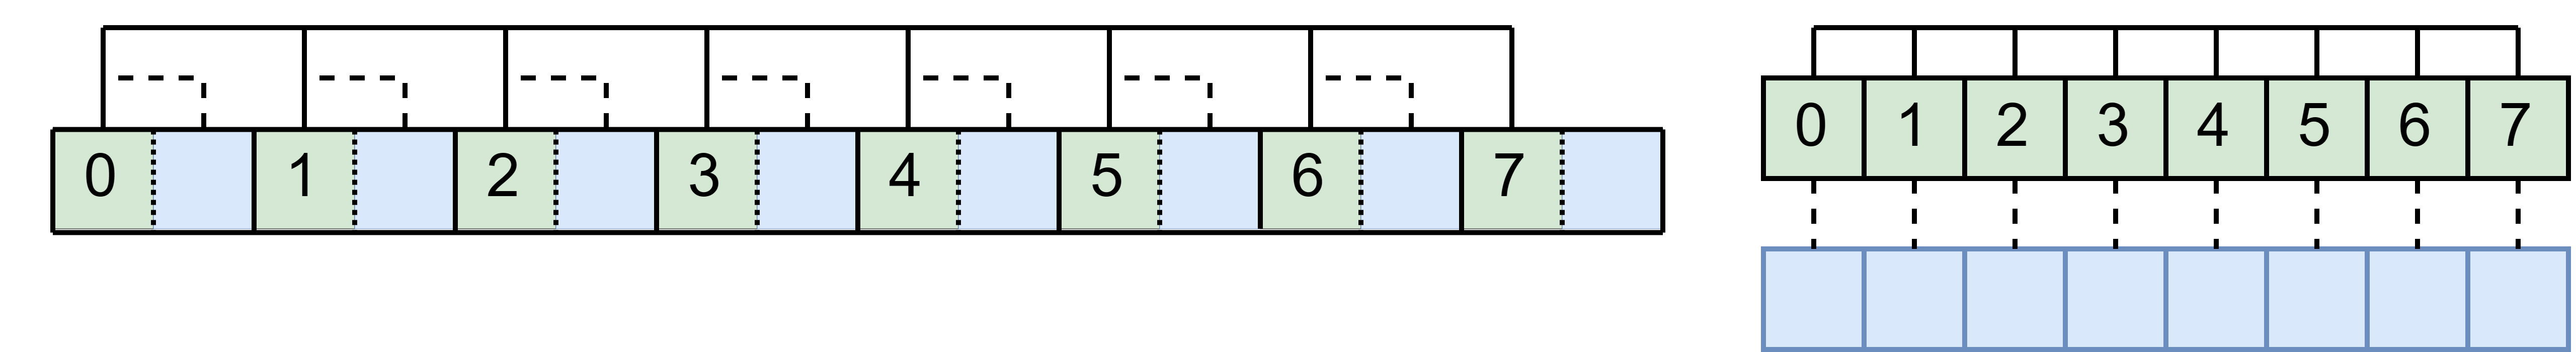
\includegraphics[scale=0.082]{soa-aos.png}
    \caption
    {
        Visual comparison between an array-of-struct collection(1) and a struct-of-array collection(2). 
        The solid lines represent indices in an array and the dotted lines denote an implicit connection that is relative to the original index.
    }
\end{figure}

Caches also operate with contiguous blocks of memory, which means spatial adjacent data within a fixed alignment are stored together.
A struct-of-array collection lends itself well to the cache, as it means the least amount of cache blocks are required irrespective of block size and alignment\footnote{Note that this is only the case when {\it all} elements in an array are operated on, which falls under the predefined context of this chapter.}.
A function that operates on a single field in an array-of-struct collection pollutes the cache with the (unused) fields, which is not an issue for the struct-of-array collection. 
In addition all memory accesses use the same linear function, a {\it constant stride} access behavior, which makes it particularly receptive to hardware cache prefetching\cite{cache-prefetching}. 

\paragraph{Access Patterns}

As the cache is finite in size, a cache block can be ejected prematurely.
Both for data within the same cache block but also when the same block is required at multiple times in the application.
In the previous chapter it was stated that a cache replacement policy is based on temporal properties, which can be leveraged to increase the chance requested data exists in the cache.
Increasing temporal locality is done by avoiding random accesses and organizing computations order when certain data is used.
This is non-trivial in iterations which access multiple indices (stencils) or computations that inherently involve random access (linked lists).
Due to the way caches operate with contiguous blocks, spatial locality of data commonly used together can also reduce the total amount of cache blocks that are required. 

\newpage

\begin{figure}[ht]
    \centering
    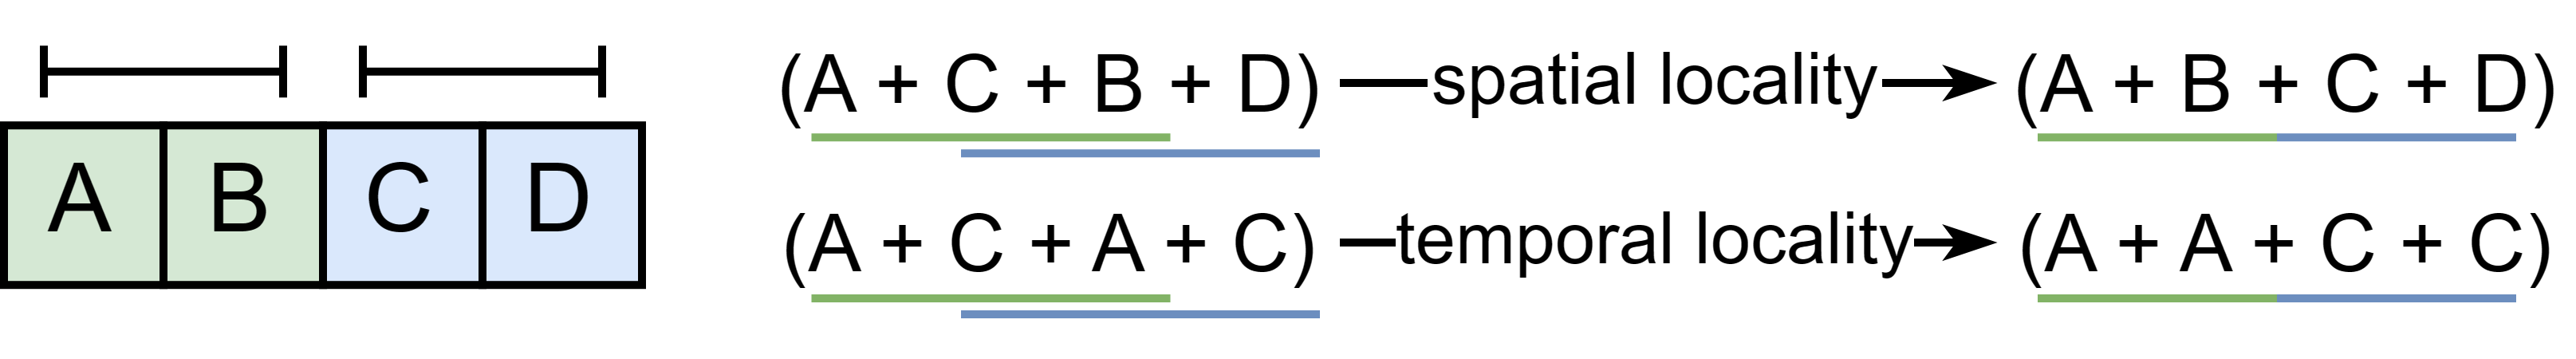
\includegraphics[scale=0.12]{temporalspatial.png}
    \caption
    {
        Comparison between temporal and spatial locality, where the data A/B and C/D will exist in different cache blocks when stored in the cache.
        The initial sequence of operations has overlapping live time of cache blocks.
        Reordering the operations can facilitate both spatial and temporal locality.
    }
\end{figure}

A way to contextualize this is by partitioning an array into multiple segments, where each segment is repeatedly iterated on and therefore cache blocks will be reused (tiling).
Cache coherence can be further improved by also accounting for shared resources, by grouping elements that use the same resource in their instruction sequence. 
This technique is explored in raytracing\cite{raytracing-reorder-ray}, where rays are sorted to exploit the fact that spatially adjacent rays likely traverse the bounding-volume-hierarchy similarly.
Avoiding redundant cache blocks is also important for multi-core processors, as it reduces the need for data to exist in multiple caches at the same time and minimizes cache reloads.

\paragraph{Branching}

Pipelining instructions is not possible when the sequence of instructions is dependant on the result of a previous instruction.
This limits instruction-level parallelism, which is solved through various ways of unconditional instruction executions\cite{instruction-level-parallelism}.
Either by discarding the computed results or by {\it flushing} the pipeline when the wrong branch is predicted, both of which intuitively have an overhead.
A compiler can eliminate\footnote{Either by proofing the branch will never be executed or by replacing the branch with a {\it conditional move} instruction, which only writes the result on true.} branches or move loop-invariant code to facilitate instruction-level parallelism\cite{assembly-optimizations}. 
These optimizations are not absolute, as an increase in instructions can pressure registers usage and the cache.  
It is also limited to instructions that cannot fail or overflow, as unconditional execution of these instructions can introduce unintentional side-effects.  

\begin{figure}[ht]
    \begin{minipage}{.5\textwidth}
        Branching is also problematic for vectorization, as all data within the instruction size must follow the same sequence of instructions.
        It can be resolved through the use of a {\it bitmask}, which can nullify parts of a result\cite{assembly-optimizations}.  
        Another notable application of unconditional execution is sequential loops, where unrolling the loop creates an opportunity to vectorize the scalar instructions.
        Automatic vectorization of loops is an active field of research, and limitations have been primarily attributed to the lack of analysis information available to compilers\cite{automatic-vectorization}. 
        This means branchless code and simplifying control flow allows the compiler to vectorize instructions in more instances.   
    \end{minipage}%
    \begin{minipage}{.5\textwidth}
        \centering
        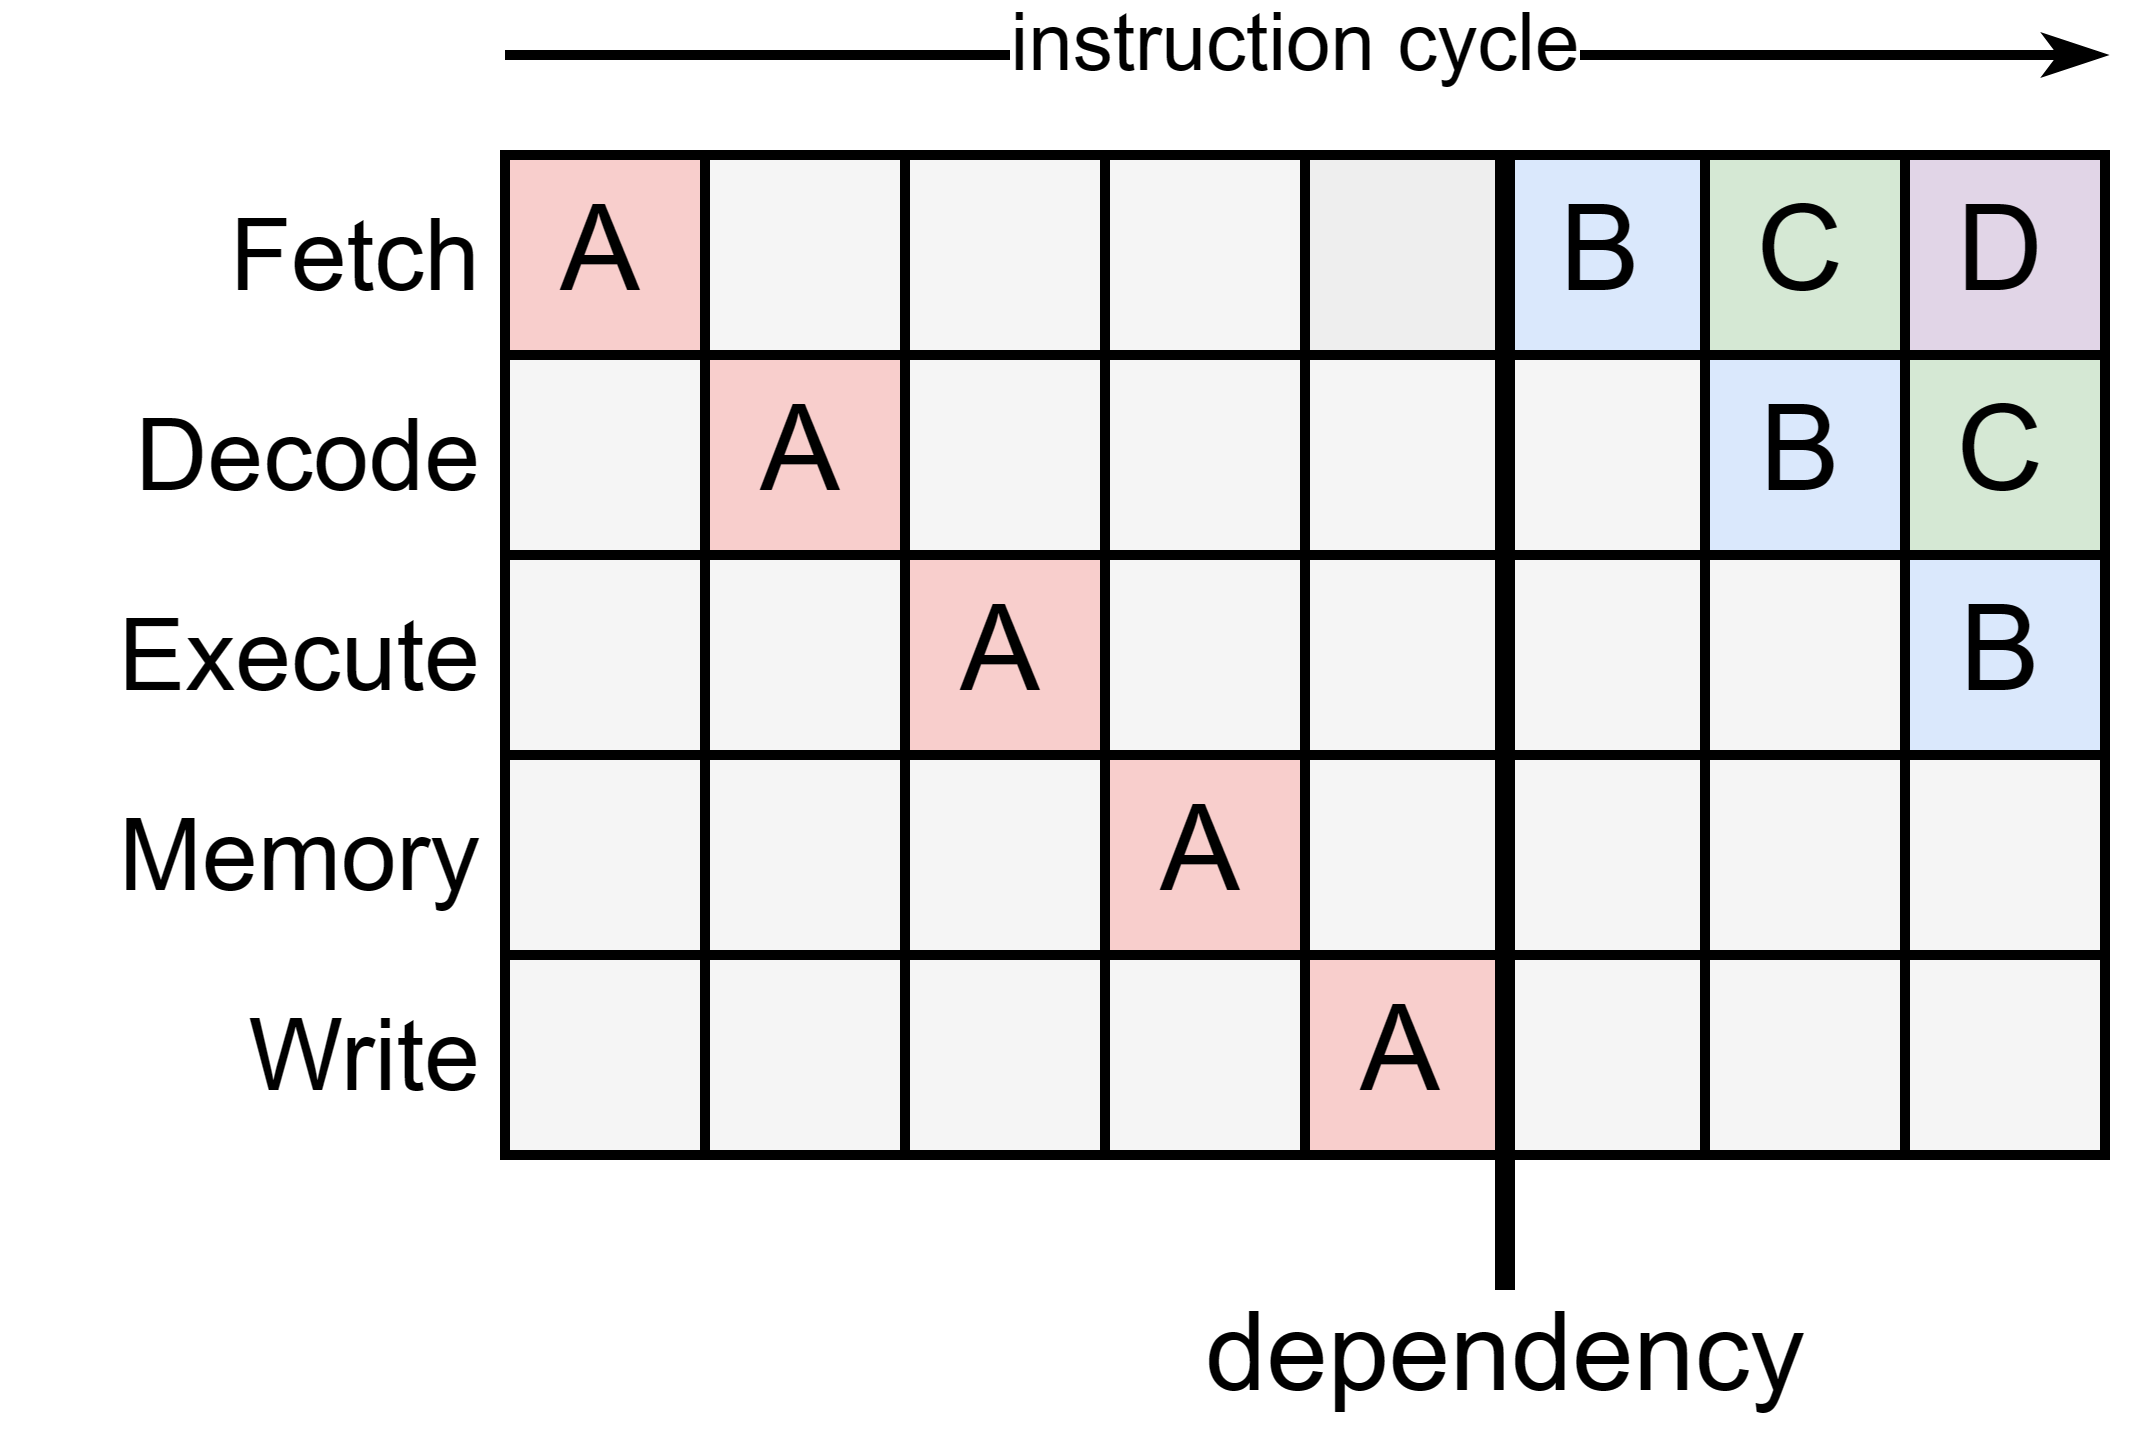
\includegraphics[scale=0.10]{UpdatedCycle.png}
        \captionsetup{margin=0.5cm}
        \captionsetup{format=plain}
        \caption
        { 
            Updated instruction-level pipeline when B is dependant on the result of A.
        }
    \end{minipage}
\end{figure}

\vspace{-0.5em}

Specialized processors where an instruction sequence is distributed over many cores are limited to executing all branches unconditionally.
This is minimized through the use of Streaming Multiprocessors (SM), which contains several cores and fetch their own instructions.
Streaming Multiprocessors operate and schedule warps, which often contain 32 threads.
When divergence between these threads occur ({\it branch divergence}) the instructions will in the general case be executed in lockstep\cite{threads-independent-scheduling}.
This means diverging execution flows are not necessarily problematic when it only occurs between different Streaming Multiprocessors, as branches that are not executed can be skipped entirely.

\newpage

\subsection{Data structures}

A fundamental aspect of computing is data structures, which is a constant overhead for all computations.
For collective operations arrays are essential; as they have a constant access time, are contiguously allocated and access can be parallelized.
Composite datatypes within arrays introduce some considerations.
One is the {\it implicit} use of parallel arrays, where each primitive datatype is stored in a distinct array.
This enables vectorization opportunities, but a random access pattern might cause additional cache blocks to be cycled between.
Since collective operations control the access pattern, parallel arrays are often a natural choice for array languages.
The consideration for both structurally and functionally distinct data, now referred to as variant, is often complex.
Variants can be represented on an individual basis (element-wise) or collectively (variant-wise).
Usage and implementations of these approaches are explored in this chapter. 
Within this chapter the assumption is made that parallel arrays are used, as they align with the intention to vectorize operations. 
The example composite datatype has type \textcolor{blue}{A}, and either has type \textcolor{red}{B} or type \textcolor{green}{C}.

\subsubsection{Element-wise}

For each element the choice of variant is represented, which introduces branching and in the general case will break vectorization.
As variants are not grouped, functions cannot iterate on a specific variant without iterating on the complete array.
The main advantage is that a variant change can be done independent of other elements, and thus can be parallelized.
A practical consideration is that each element in an array must be structurally the same, that is they occupy the same memory space.
This is a limitation which enforces that each index can determine the location of an element. 
For parallel arrays this restriction applies for all arrays individually\cite{accelerate-sum-types}.

\paragraph{Memory Representation}

Memory instructions operate on fixed boundaries, which means operations that overlap these boundaries require additional but strictly unnecessary instructions.
A natural alignment of a datatype is achieved by aligning all types according to the instructions that access them.
Many compilers introduce {\it padding} to enforce natural alignment for all the types within the structure.
While computational efficient, the alternative of {\it packing} types together can be preferred for a smaller memory footprint.  

\begin{verbatim}

    struct PackedData // 8 bytes
    {
        char  name;         // 1 byte
        int   node;         // 4 bytes
        short identifier;   // 2 bytes
        byte  alignment[1]; // 1 byte
    };

    struct PaddedData // 12 bytes
    {
        char  name;         // 1 byte
        byte  padding[3];   // 3 bytes
        int   node;         // 4 bytes
        short identifier;   // 2 bytes
        byte  alignment[2]; // 2 bytes
    };    

\end{verbatim}

Parallel arrays (Struct of Arrays) have a natural alignment by default as they contain primitives types, which are naturally aligned.
General purpose languages often default to the Array of Struct, while data-parallel applications use the Struct of Arrays representation.
A zero-cost abstraction that can ergonomically switch between these constructs is non-trivial.
An interface to index access with an intermediate structure can break automatic vectorization\cite{abstraction-vectorization}. 
In addition the different internal representations must be statically definable and able to be handled by the data structures.
Many C++ libraries utilize {\it class templates} to achieve this\cite{abstraction-vectorization}.

\paragraph{Tagged Union}

Multiple variants can be represented through a tag and a fixed size data component with multiple representations, so called {\it union}.
The tag is used to identify the current representation of the union. 
A naive implementation creates an array for each field of each variant, which means the memory usage is cumulative for each variant. 
A compact tagged union overlaps fields of variants, as only one representation can be valid at a time.
This can in theory reduce the size to the largest variant and the accompanied tag, but this is complicated due to alignment requirements\cite{accelerate-sum-types}.

\begin{figure}[ht]
    \centering
    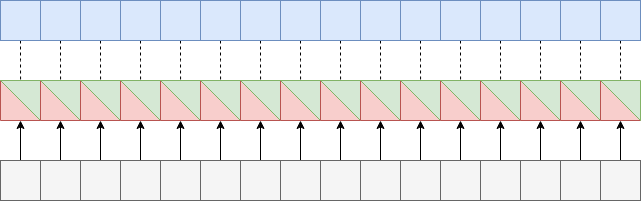
\includegraphics[scale=0.4]{taggedunion}
    \caption{ index implicit and tag (gray) identify the data representation }
\end{figure}

\newpage

\paragraph{Tagged Pointer}

Another way to comply with elements being structurally the same is to use a form of indirection, in this case a pointer to memory.
The indirection allows variants to escape the uniform size restriction, but there are several notable complications.
General complications around pointers, such as being unsafe to operate on and complicating garbage collection apply.
In addition, pointers that point to the same data (alias) can prevent parallelization due to possible race conditions.
These can be partly solved through language constructs; such as smart pointers, immutable data or abstracting the use of pointers altogether.

\begin{figure}[ht]
    \centering
    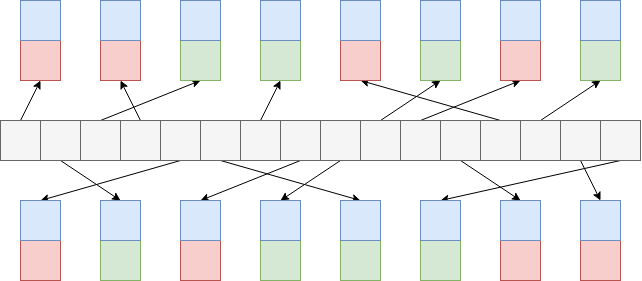
\includegraphics[scale=0.4]{taggedpointer}
    \caption{ tag and pointer (gray) identify the location and representation. }
\end{figure}

The key issue is that a change in variant requires new data to be allocated and the pointer to be adjusted.
This allocation means there is no guarantee that the data is contiguous, which in addition to the required branching prevents any vectorization efforts.
The indirection and fragmented memory is also problematic for cache efficiency, as it is unpredictable and a cache block is not used effectively.

\newpage

\paragraph{Entity}

A notable observation is that the re-allocation of a variant change causes the data to be not contiguous, not the indirection in itself.
This can be illustrated through a hash table data structure, where a key is mapped to a value within an array (bucket).
Any collective operation on the hash table can be vectorized by disregarding the hashing and using the internal array directly, as computations are inherently independent and order is irrelevant.   

\begin{figure}[ht]
    \centering
    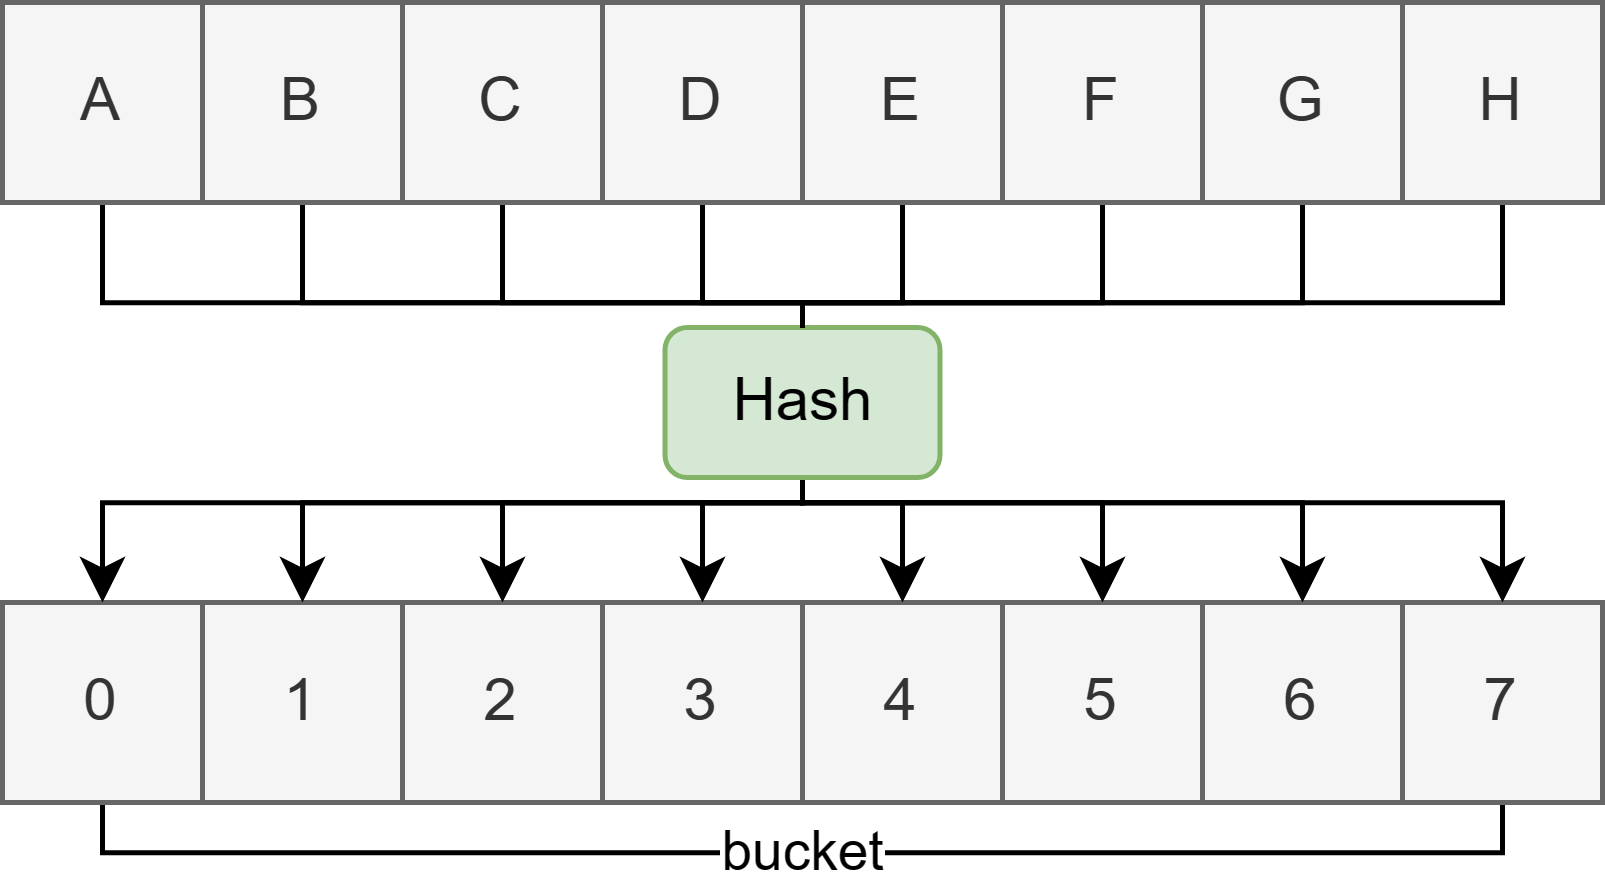
\includegraphics[scale=0.1]{hashtable}
    %\caption{ hash table }
\end{figure}

Entities within the ECS pattern function similarly, a form of indirection that is not used by the collective operations. 
Represented as a single heterogeneous array, which internally consists of several variant-wise collections. 
It will mean that variant choice is not {\it directly} represented on an element basis, which has several implications.

\begin{itemize}
    \item [Stable] 
The same entity is not guaranteed to refer to the same data, the entity is no longer stable across structural changes.
The reverse also holds, the data is not guaranteed to have the same entity along iterations.
This can solved by tracking the location of entities {\it or} annotating the data with their entity. 
These approaches can be complementary for performance reasons, but they are collectively isomorphic\footnote{A single entity cannot identify the data in constant time, without an array of pointers. A data element cannot identify the entity in constant time, without the entity as data. } through gather and scatter operations. 

\begin{figure}[ht]
    \centering
    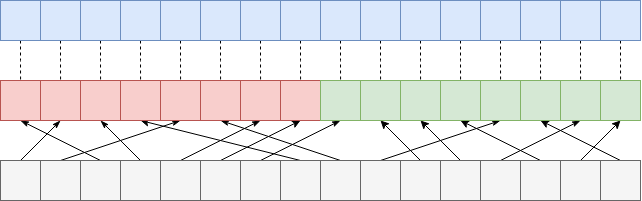
\includegraphics[scale=0.3]{stable1}
    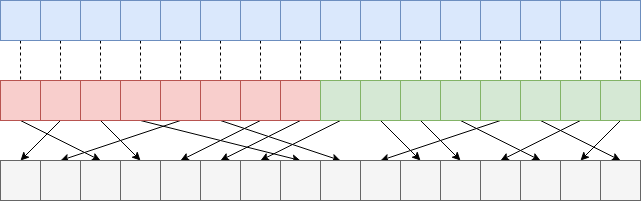
\includegraphics[scale=0.3]{stable2}
    \caption{ persistent array with indirection (1) or annotate the data with their index (2). }
\end{figure}

For many array operations stableness is excessive, as it means data is discriminated on the basis of their index. 
The implicit connection that data with the same index has can be represented through a (temporary) datatype.

    \item [Independent]
Elements can no longer change their variant independently of other elements, which can be problematic for parallelism.
Depending on the way variants are grouped, there can also be a significant cost associated with regrouping variants.
This can be minimized by delaying structural changes indefinitely, by using a tagged union approach.
Regrouping variants is a performance consideration between the cost of regrouping and having to branch for future iterations.
\end{itemize}    

\newpage

\subsubsection{Variant-wise}

Grouping variants means all data is uniform, contiguously allocated and there exist no inherit branching within the same grouping of variants.
This can be achieved through an array for each variant, but also grouping {\it within} the same array and using segment descriptors.
The latter is effectively an untagged union, where the representation is determined by the index within the array.
Both allow instructions to be vectorized, but there exist several other considerations.

\begin{itemize}
    \item [grouping]
    As stated in the previous section, regrouping variants to a variant-wise collection is a performance consideration.
    When variants are stored in separate arrays, the amount of a certain variant must be known before allocation.
    When this is dependant on a computation, it can be retrieved through an additional scan or atomically\footnote{Atomic instructions prevent interruptions by other processes and are thread-safe.} counting any structural change, which adds an overhead.
    This is not required for a singular array if the total remains the same.

    \item [immutable]
    An important consideration for purely functional languages is that values, and therefore arrays, are to be considered immutable.
    This means that {\it{updating}} parts of an array efficiently is non-trivial.
    It must be proven that the array before update will never be used again, otherwise both arrays must co-exist in memory.
    This is inefficient for small updates and grows the necessity to {\it destructively update}\cite{destructive-update-array}.

    \item[automatic]
    Most compilers support automatic vectorization of iterations with flexible bounds, where the final leftover iteration is not vectorized.  
    This overhead can be a significant when the loop is extensively unrolled.
    This is minimized through epilogue vectorization, which (re-)applies loop vectorization to the remaining scalar code.
    In practice data must be aligned along specific byte boundaries to be vectorized, which is challenging for (dynamic) regions within an array and not always analyzed by compilers\cite{automatic-vectorization}.

    \item [operable]
    An undiscussed benefit of parallel arrays is that fields can be operated on independent of other fields, as they are distinct arrays.
    This is also possible for {\it regions} within an array, but this is less trivial and often requires explicit support in array languages\cite{accelerate-independent-regions}. 


\end{itemize}

\begin{figure}[ht]
    \centering
    \includegraphics[scale=0.3]{variant1}
    \hspace{10pt}
    \includegraphics[scale=0.3]{variant2}
    \caption{distinct arrays (1) or distributed in a single array (2)}
\end{figure}

\begin{figure}[ht]
    \centering
    \includegraphics[scale=0.3]{variant3}
    \caption{combination of both approaches}
\end{figure}

\newpage

\section{Interface}

A preliminary conclusion of the previous chapter is that a performant internal representation cannot be deducted from a mere theoretical framework.
With this in mind it is important for high performance oriented applications to be flexible with the internal representation of datatypes.
This is important for both composite data types and data structures.
Within this chapter a modular interface is explored around iterating on collections of non-uniform data.

\subsection{Paradigm}

As discussed in the data structures section, there are two internal representations for collections of non-uniform data.
Variants of a particular type are stored either element-wise or variant-wise.
There are several considerations for a data structure that is agnostic to if it stores non-uniform data in element-wise or a variant-wise way.
A variant-wise collection can operate on only the relevant variants, while an element-wise is forced to discover that at runtime.
To avoid redundant iterations for variant-wise collections, a function must be able to be defined on the most specific subset of all variants.
For element-wise collection the amount of variants must be finite and no large discrepancies can exist between the size of all the variants.


\begin{figure}[ht]
    \centering
    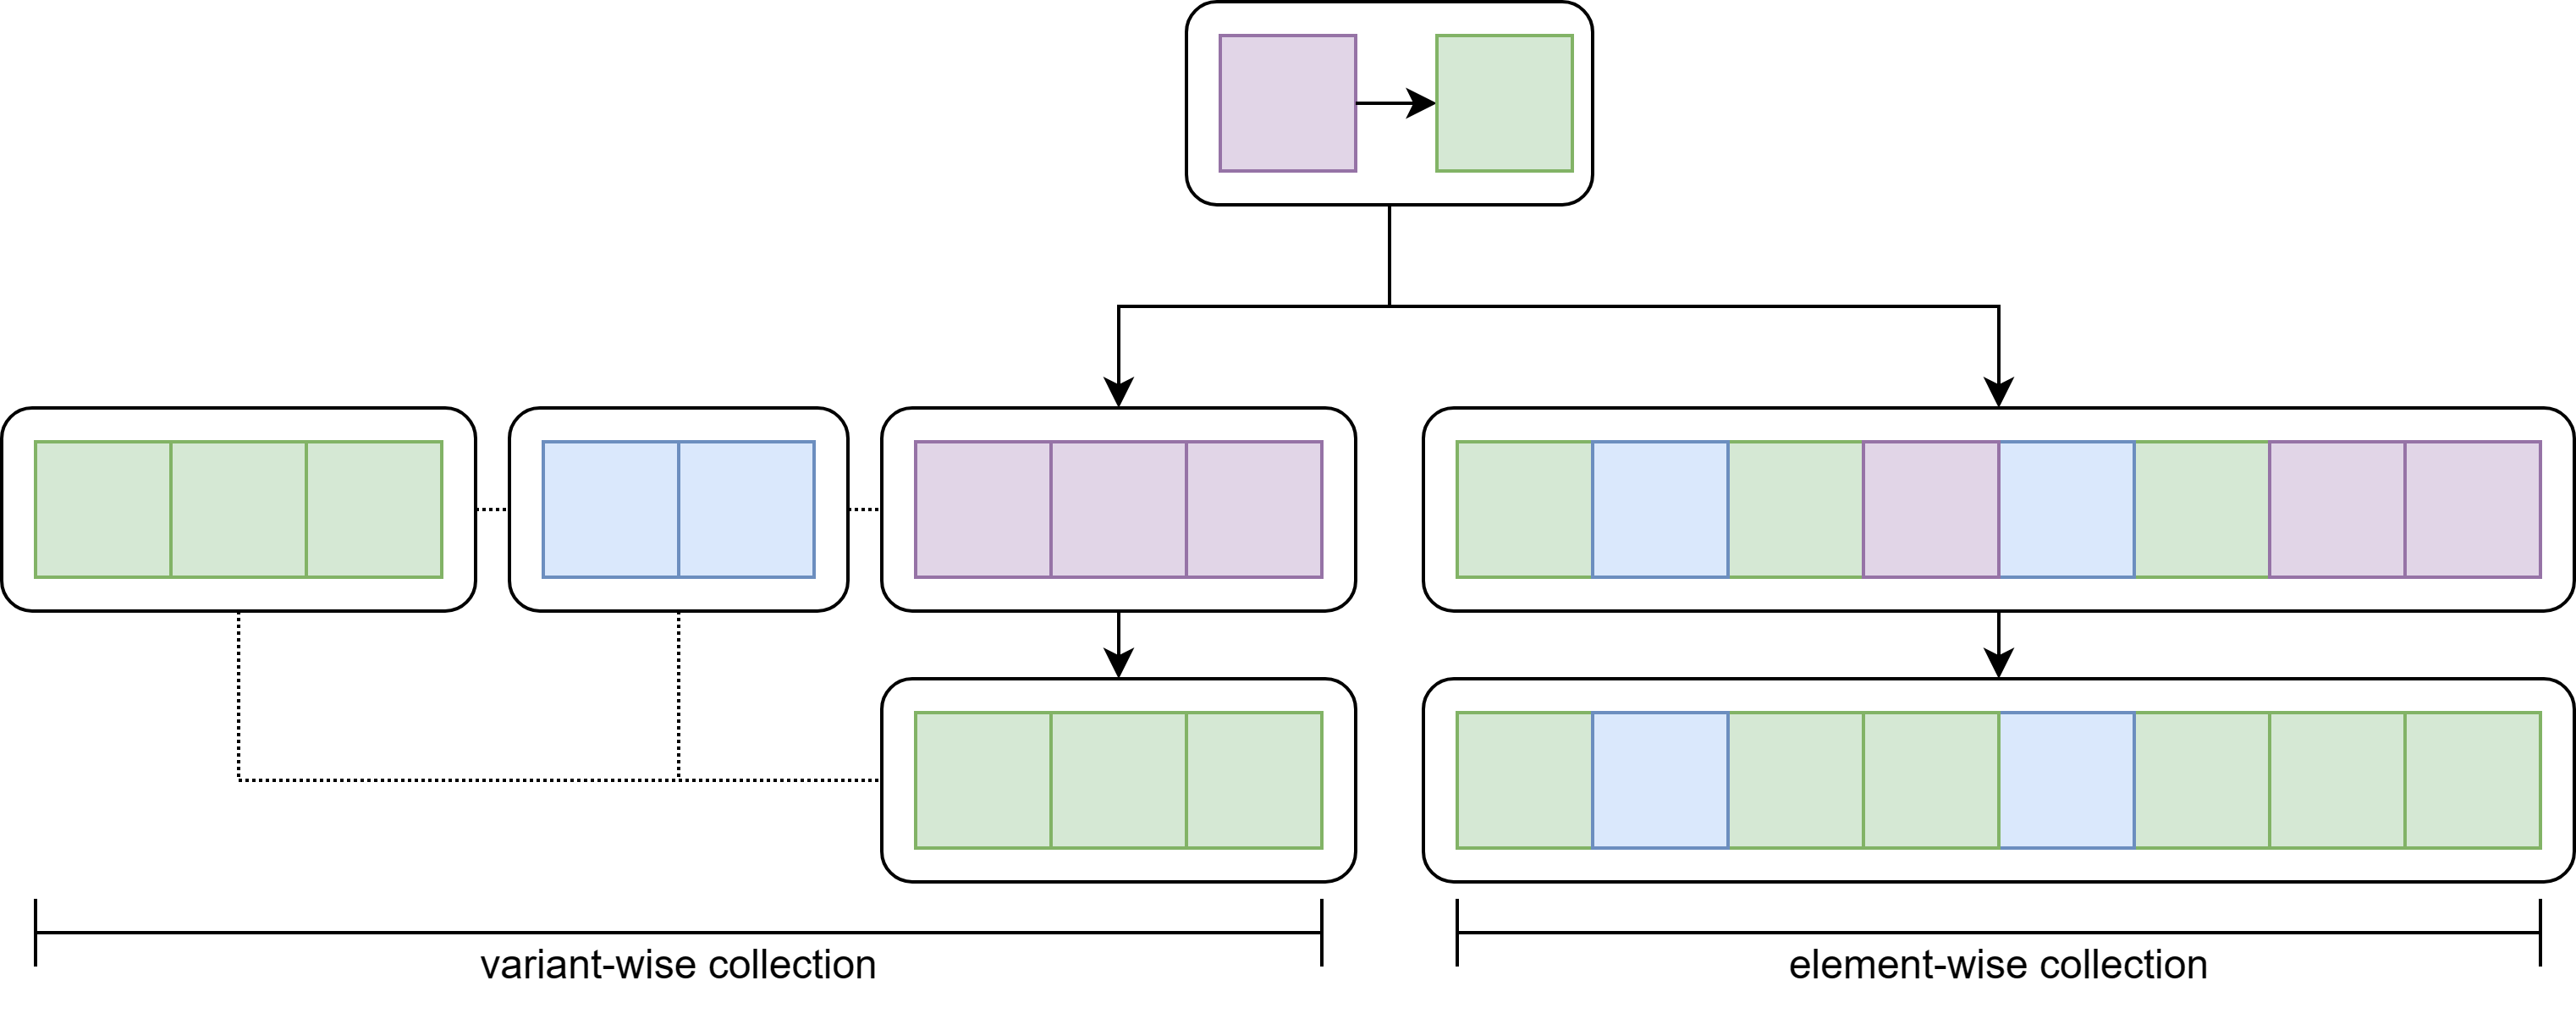
\includegraphics[scale=0.1]{paradigm.png}
    \caption{A non-exhaustive function can skip a significant amount of work when non-uniform data is stored in a variant-wise collection, while this is problematic for an element-wise collection. }
\end{figure}

For variant-wise collections the ECS-pattern will be used as reference.
The first section goes into how the ECS-pattern collectively operates on only some variants.
For element-wise collections Algebraic Data Types (ADTs) are used to safely discriminate between multiple variants as element. 
The second section utilizes structurally typed ADTs to create an efficient interface for a variant-wise and element-wise collection.  

\newpage

\subsubsection{Entity-Component-System}

The ECS pattern is arguably a reaction to the prevalence of object-oriented languages within game engines.
The premise is to organizes game-logic within functions rather than data, where the relation between data is flexible\cite{ecs-origin}.
In contrast to inheritance, where relations are statically determined and game-logic is embedded within an predetermined hierarchy.
The pattern is often combined with data-oriented design and is used to be able to implicitly exploit data-parallelism in general purpose languages. 
While there exist many implementations of the pattern in many languages, the principles remain similar.  

\paragraph{Components}
A component is the smallest addressable type within the pattern.
Examples of components are \type{Position} and \type{Velocity}, which together represent movement.
Components are generally value types to avoid race conditions when using data-parallelism.
Some implementations allow for a (readonly) reference component that is shared along multiple instances.
A shared \type{Mesh} component prevents redundant geometry to be stored by referencing it.

\paragraph{Entity}
An entity is idiomatically a set of components.
A movable entity has the \type{Position} and \type{Velocity} components, while an immovable entity only has the \type{Position} component.
Adding and removing components is done at runtime and there is no predetermined relation between any of the components.   
Any immovable entity can be made movable by attaching the \type{Velocity} component at runtime.

\paragraph{Systems}
A system operates on all entities that match a specific set of components.
The \type{Movement} system will operate on all movable entities, irrespective of any other attached components.
Systems are effectively global functions, which operate only on specific variants of the more general entity type. 
This allows for a variant-wise collection of entities, which most ECS implementations enforce to implicitly create performant vectorized code.

\begin{figure}[ht]
    \centering
    \includegraphics[scale=0.2]{ecs}
    \caption{ conceptual entity-component-system representation of systems }
\end{figure}

The ECS design pattern is arguably inherently imperative, as structural changes to entities are done imperatively.
Apecs, an ECS library in Haskell, achieves this imperative style through monads\cite{ecs-apecs}.
The ECS pattern makes element-wise collections infeasible, as there is no type-safe way to restrict the possible amount of structural changes to an entity.
This is inherit to the pattern, as any component can be attached to any entity.
Implementations circumvent this limitation by allowing components to be enabled and disabled through a tag.
Disabling a component changes the {\it type} of an entity but the internal representation remains the same.
An analogy can be made to a non-deduplicated tagged union that is explicit in the variants it holds.

\newpage

\subsubsection{Algebraic Data Type}

Functional languages handle tagged unions safely through algebraic data types (ADTs).
A product type (x) is the combination of datatypes, while a sum type (+) is the alternation between datatypes.
It is often useful to discriminate between variations of a datatype, which is generally done through a data constructor. 

\begin{verbatim}
    
    data Maybe a = Just a | Nothing
    
\end{verbatim}

Deconstructing an algebraic data type is done by pattern matching on a data constructor.
The pattern match can exhaustively match on all variants, as the data constructors of variants are known at compile-time.
It can be seen as a native control-flow mechanism that ensures only the operations on the active variant are applied.

\begin{verbatim}
    
    fmap :: (a -> b) -> Maybe a -> Maybe b
    fmap f (Just a) = Just (f a)
    fmap f Nothing  = Nothing
    
\end{verbatim}

In Haskell, algebraic data types are distinguishable by name (nominally typed) and therefore explicitly declared.
This means data constructors are local to the declared type and pattern matching happens within the same type.
The type signature of the \type{fmap} function provides no information on the potential structural change of a datatype.
It is possible to return \type{Nothing} for both cases\footnote{\type{Just b} is not possible as it can only be inferred through \type{Just a} and the \type{a -> b} function.}.
A function that takes \type{Just a} and returns \type{Just b} ensures that the {\it collective identity} is preserved in a collective operation, irrespective of the data transformation.
This exact definition is not possible due to being nominally typed, as \type{Just a} is not a type but a data constructor under the type \type{Maybe a}. 
In some cases, such as a safe division function, the introduced branching is inherit to the function and is now made explicit in the type definition.   

\begin{verbatim}

    fmap :: (a -> b) -> Just a -> Just b
    fmap f (Just a) = Just (f a)

    divide :: Int -> Int -> (Just Int | Nothing)
    divide _ 0 = Nothing
    divide n m = Just (n `div` m)
    
\end{verbatim}

In this case a function is defined on the structure of a type, the data constructor of algebraic data types.
\type{Maybe a} is now an alias for the mutually exclusive relationship \type{Just a | Nothing}, rather than a unique and standalone type. 
This generalizes variance to be between all types.
OCaml calls these {\it polymorphic variants}\footnote{OCaml also implements nominally typed sum types, so called {\it variants}.}, while other functional languages generally refer to them as {\it extensible} or {\it open sum types}.
A motivating example is that a collection of \type{Maybe a} can be an element-wise collection or two variant-wise collections of \type{Just a} and \type{Nothing}\footnote{As \type{Nothing} does not hold data, a size descriptor is sufficient.}.
While the former involves branching for \type{fmap}, the latter can ignore the \type{Nothing} collection and vectorize the \type{fmap} function.
This flexibility aligns with the intention to create a modular system that is agnostic to the internal representation.

\newpage

\subsection{Type-level programming}

In the previous section an interface that is agnostic to the variant-wise and element-wise collection is proposed.
This demands defining efficient intermediate internal representations for all possible variant combinations, which defeats the purpose of ergonomic switching between representations.
Statically deriving an internal representation is impossible or restricted to predetermined parameters in most languages.
Some high-performance libraries circumvent this restriction by meta-programming or custom data layouts\cite{llama}.
A customizable and type-safe solution is type-level programming, which will be explored in this chapter.

\subsubsection{Kinds}

A value is categorized by types, while a type is categorized by {\it kinds}.
This is relevant when discussing type constructors, where each constructor with a different arity has a distinguishable kind.
A well known exposition of type constructors are parametric polymorphic data types, which take type variables as argument.
While a lot of languages support polymorphic data types, the concept of kinds is not evident as only concrete types are able to be used for arguments.
Haskell supports higher-kinded types, which are analogous to higher-order functions for types, which makes kinds apparent to the user.

\begin{verbatim}
    2.5f         :: Float
    Float        :: *
    Option a     :: * -> *
    Option Float :: *
    Apply f x    :: (* -> *) -> * -> *
\end{verbatim}

Type constructors can be used to encode data statically, such as Peano numbers.
The parametric \type{Succ a} and \type{Nil} types are axioms that can be used to construct a natural number on the type-level.
By default these exist in a open universe, which means ill-formed expressions can be created.
On the type-level this can be resolved by Generalized Algebraic Data Types (GADTs), implemented in Haskell as an extension.
It allows the type variables of constructors to diverge from the more general type.

\begin{verbatim}
    // open universe where 'a' can be anything
    data Succ a
    data Nil

    // closed universe under the phantom type 'a'
    data Natural a where
        Succ :: Natural b -> Natural (Natural b)
        Nil  :: Natural ()
\end{verbatim}

The consequence is that deconstructing a GADT will refine the type.
This can be used to construct evidence of certain properties by pattern matching on data constructors.
An observation is that this is a categorization of types, similar to how the kind \type{*} represents all concrete types.
The \type{DataKind} extension promote types to the kind-level and constructors to the type-level. 
The kind \type{Natural} includes the types \type{Succ (a :: Natural)} and \type{Nil}.
It both creates a closed universe and allows other type constructors to expect the more precise kind \type{Natural}.
A limitation is that the construction of the type, which is needed for arithmetic operations, is guarded by the definition of \type{Natural}.

\begin{verbatim}
    data Natural = Succ Natural | Nil | Add Natural Natural | Minus Natural Natural
\end{verbatim}

On the value-level this is solved through functions that transform their input into another output type.
Translated to the type-level it means type-level functions that transform an input kind into an output kind.

\newpage

\subsubsection{Type Family}

A way to approach type-level functions is to see it as a type dependent on the instantiation of a type variable.
This is akin to functions in type classes, where type-indexing allows functions to be overloaded.
Haskell reuses this functionality for types, categorizable as {\it associated types}\cite{associated-types}.
This is particularly useful for domain-specific languages, as an instance can have a specialized return type.
Accelerate uses the \type{Elt} class to create a mapping between surface types and the internal representation.

\begin{verbatim}
    class (Elt a) where
        type EltR a :: *
        toElt       :: a -> EltR a
        fromElt     :: EltR a -> a
\end{verbatim}

While these integrate well with type classes, type families is the terminology for the standalone concept.
A \type{data family} has unique types associated with the type, while a \type{type family} is merely the type synonym equivalent.
In some cases this is insufficient to represent a function, as the type checker is unsure which instance to use.
This is the case when the function has a more general default case which will always match.
A closed type family attempts the instances in order of definition, which expresses itself in being able to pattern match on types.

\begin{verbatim}
    type family Elem a (bs :: [b]) :: Bool where
        Elem x '[]       = False        -- no
        Elem x (x : ys)  = True         -- yes
        Elem x (y : ys)  = Elem x ys    -- no, but recurse
\end{verbatim}

In this example the variable \type{y} can be \type{x}, which means the second and third instance are overlapping with each other.
A closed type-family resolves this by attempting the more specific case of \type{x = x} first.
An annoying limitation is that type families in Haskell cannot be partially applied, which means a lot of boilerplate is required to capture more complex functions.
It cannot be partially applied due to partially applied type synonyms requiring higher-order unification, which is currently not supported in Haskell.

\subsubsection{Interface}

Type-level functions allow for computation of types, and as such a way to easily construct multiple representations for a single type.
The process of constructing multiple representations can be captured within a single datatype.

\begin{verbatim}
    data Variant (constructor :: [variant] -> *) (variants :: [variant])
\end{verbatim}

The data type \type{Variant} takes two type variables, a higher-kinded construction type and a promoted list type.
The constructor takes the promoted list and transforms it into a concrete type.
As type families cannot be partially applied, a data family is used to create a constructor.

\begin{verbatim}
    data family Constructor argument :: [variant] -> *

    type V argument (variants :: [variant]) = V (Constructor argument) variants
\end{verbatim}

An instance of the constructor data family constructs a unique type based on some type argument.
An example variant type is \type{V Compact [Int, Float, Bool]}, where \type{Compact} is an (empty) descriptive datatype.
The \type{Compact} type is associated with the constructed type within the data family.
 
\newpage

\subsubsection{Type Structure}

With closed type families it is possible to derive compact layouts for multiple variants of a type.
As a memory layout only concerns itself with the bit sizes of types, the intermediate structure will be the previously discussed natural number.
The \type{DataKinds} extension natively supports the \type{Nat} kind with arithmetic expressions and literals for syntax.
While mapping of primitive types to their corresponding natural number is trivial, this is not the case for user-defined datatypes.

\begin{verbatim}
    type family BitSize (a :: *) :: Nat where
        BitSize Word8  = 8
        BitSize Custom = ?
\end{verbatim}

It is not possible to statically derive the bit size of the \type{Custom} type within the type family.
For this the types of which \type{Custom} is composed must be known to the type family.
This means the structure of the type must be apparent to the type family.
One way to approach this is to use a kind more specific then \type{*} that is explicit in the composition, such as the \type{Natural} kind but for all datatypes.
Another way is to enforce an implicit constraint by ensuring the type can be constructed with a particular GADT.
The latter is used by Accelerate where the \type{TupR} constructor ensures that the type is composed of only units, singles and pairs.
The function \type{eltR} enforces this by requiring the associated type \type{EltR a} to have a mapping to the \type{TupR} type\footnote{Note this can circumvented by merely returning a bottom type such as \type{undefined}, which will only be detected when using the value. }. 
The GADT approach is preferable when access to the structure on the value-level is needed, which is the case for future datatype generic programming endeavors.

\begin{verbatim}
    class (Elt a) where
        type EltR a :: *
        eltR        :: TupR (EltR a)

    data TupR v where
        TupRunit   ::                     TupR ()
        TupRsingle :: a                -> TupR a
        TupRpair   :: TupR a -> TupR b -> TupR (a, b)
\end{verbatim}

A simple example to demonstrate the explicit structure is to convert tuples of \type{Word8} to a single type. 
In Accelerate each primitive type in a tuple is spread out over multiple arrays, which means this type-family enables an Array of Struct representation for such a tuple.

\begin{verbatim}
    type family ToBitSize (a :: *) :: Nat where
        ToBitSize (a, b) = ToBitSize a + ToBitSize b 
        ToBitSize ()     = 0                   
        ToBitSize Word8  = 8 

    type family FromBitSize (a :: Nat) :: * where
        FromBitSize 0    = ()
        FromBitSize 8    = Word8
        FromBitSize ...  = Word...
\end{verbatim}

In Accelerate the embedded representation is the one relevant for optimizations.
All type-functions therefore operate on the embedded representation, the type associated with \type{EltR}.
It is impossible to construct such type outside the \type{Elt} class.
A solution is to automatically derive the \type{EltR} class for a set of types with a fixed representation, such as tuples. 
A return type with a fixed representation means that all computed representations will implement the \type{Elt} class. 
It is now possible to ergonomically define many internal representations for embedded representations.

\newpage

\subsubsection{Layout}

While the tools are there to generically construct intermediate representations, it is not trivial to create a single performant solution.
Within this section a modular interface is proposed which allows for ergonomic switching between internal representations of multiple variants.
The most general intermediate structure of a composite datatype is a collection with the size in bits of each field in the datatype.
This removes both hierarchy and type identity, which makes it is easier to reason about the layout of a datatype.
The representation does preserve performance critical information about the way data is retrieved from the internal representation.

\begin{verbatim}
    type family FieldSizes (a :: *) :: [Nat] where
        FieldSizes (a, b)   = FieldSizes a ++ FieldSizes b 
        FieldSizes ()       = '[]                   
        FieldSizes a        = ToBitSize a : '[]
\end{verbatim}

For simplicity the kind \type{[]}, the promoted list type, is used to denote all possible variants of a certain type.
With closed type-families it is possible to define all relevant operations on lists.
The definition of these are similar to their value-level counterparts without any partial application.
With these operations it is possible to define a type-level union that creates a compact deduplicated union.
The \type{FieldSizes} function returns a list of natural numbers, the size for each individual field in a tuple. 
The \type{BitSizeUnion} recursively adds the unique elements for each datatype, such that all fields map to a distinct element.
This is achieved by removing the element from the comparison list once it has been matched.

\begin{verbatim}
    type family Difference (a :: [r]) (b :: [r]) :: [r] where
        Difference '[]      bs = bs
        Difference (a : as) bs = a : Difference as (RemoveOne a bs)

    type family BitSizeUnion (a :: [Nat]) (b :: [r]) :: [Nat] where
        BitSizeUnion xs  '[]      = xs
        BitSizeUnion xs  (y : ys) = BitSizeUnion (Difference xs (BitSizes (EltR y))) ys
\end{verbatim}

While strictly speaking the representation is compact, it deduplicates when the bit size of the primitive type is of equal size.
This is very safe, as there is no inherit performance cost to operating on types with the same size.
This is not necessarily the case for types stored in a larger type, or even a type spread out over multiple types.
In some memory-bound cases this approach can still be preferable.
An efficient implementation requires type-level sorting, to avoid a scenario where the smallest type is inserted into the largest type.
A naive sorting algorithm is quite trivial to implement, by inserting all elements into their respective position. 

\begin{verbatim}
    type family Sort (types :: [Nat]) :: [Nat] where
        Sort '[]      = '[]
        Sort (x : xs) = Insert x (Sort xs)
\end{verbatim}

The derivation of such a compact layout is not particularly complex, as it is similar to the deduplication approach but with multiple stages.
Each step increasing the perceived performance cost of the merge and avoiding a local optimum solution by unifying large datatypes first. 
The complexities of such layout exist with generically operating on such a layout. 

\newpage

\subsection{Datatype-Generic programming}

In the previous chapter we established a way to compute a wide-range of internal representations for a set of variants.
It is not ergonomically viable to write insertion and extraction functions for all the different internal representations. 
As users can create their own representations there is no closed system, so mapping between all datatypes must be handled.
This can be done through datatype-generic programming, which parametrizes on the composition of a datatype\cite{datatype-generic-programming}. 
A mapping must be isomorphic, such that all information is preserved between construction and deconstruction of the union.
This is not possible for all possible pairings, as the variant must be smaller or equal to the size of the representation.
Within the first section a type-level way to prove valid pairings is explored, essential for supporting user-defined datatypes.
The second section goes onto the theory of datatype-generic programming, which is used for an implementation of a datatype-generic framework in the third section.

\subsubsection{Verifying}

A variant must be smaller or equal to the representation.
A variant that is larger than its representation loses information when constructing and deconstructing, which means type safety is breached.
While it is possible to ensure that the computation of the representation is always larger than all the variants, this is a risky construction.
It limits users extensibility and does not catch flaws within the type computation code. 
A modular implementation requires an independent method that ensures the variant is smaller than its representation.
The \type{Constraint} kind can be used to restrict the construction to larger or equal types.
Constraints occur on the left-hand side and are generally constructed through type-classes to enforce a general interface.
A relevant example is ensuring that our newly computed representation has a mapping to the embedded representation.

\begin{verbatim}
    class (Elt a) where
        type EltR a :: *

    instance (Elt (constructor types)) => Elt (Variant constructor types) where
\end{verbatim}

In the type-level programming chapter we already achieved a way to determine the size of any type as kind \type{Nat}.
Fortunately the native \type{Nat} type already has several comparison operators with the kind \type{Nat -> Nat -> Constraint}.
A simple but functional constraint is the \type{<=} operator.
While it does omit performance considerations, this is required to support a wide-range of representations.
The \type{IsVariant} class has a default implementation but can be extended by the user to support unsafe variants, such as sentinel values.
The data-type generic programming part pertains to implementing the default \type{construct} and \type{destruct} functions.

\begin{verbatim}
    class (Elt v, Elt t, BitSize v <= BitSize t) => IsVariant v t where

        construct :: Exp v -> Exp t
        construct = ...

        destruct  :: Exp t -> Exp v
        destruct = ...
\end{verbatim}

\newpage

\subsubsection{Theory}

Before looking into how \type{construct} and \type{destruct} are implemented concretely, it is essential to understand the problem datatype-generic programming is attempting to solve. 
Paradoxically variant types are best to illustrate the problem, coined the {\it expression problem}\cite{expression-problem}.
Extending the variants within the \type{Color} type means all functions that pattern match on \type{Color} must be changed. 
This can be resolved by having a general interface, but extending the behavior of this interface requires all types that implement the interface to change. 

\begin{verbatim}
    data Color = Red | Green | Blue             class ColorInterface a  
                                                    transform :: a -> a
    transform :: Color -> Color
    transform Red   = ...                       instance ColorInterface Red where
    transform Green = ...                           transform :: Red -> Red
    transform Blue  = ...                           transform = ...
\end{verbatim}

The impact of the {\it expression problem} can be minimized through several methods. 
Some argue that polymorphic variants fit within this category themselves, as it separates pattern matching with the underlying data\cite{polymorphic-variants-expression-problem}.
In our case we have chosen for the representations to be extensible, which requires behavior to be defined for each possible representation.
Both constructing and deconstructing the variant type into a specific variant.
The possible datatypes is an infinite domain, which can be made finite by considering that all composite types can be reduced to primitive types.
Datatype-generic programming utilizes the inherit concept of composition in programming languages to operate on any type.
This is sufficient to generically operate on the multiple representations, as the semantics of the type are irrelevant for constructing and deconstructing the variant type.
It requires access to the composition of a type, which is often not natively supported in programming languages.
While Haskell does support datatype-generic programming, we do not operate directly on native Haskell types.
An implementation through native Haskell types, which Accelerate currently uses for sum types, is restrictive.
This is apparent when attempting to implement structurally typed sum types or more complex representations generically\cite{accelerate-sum-types}.
This is caused due to the \type{Elt} class requiring a direct mapping to the Haskell equivalent. 
The translation layer remains essential, but can be implemented with the help of the standalone implementation.
Operating directly on embedded types results in a more targeted and adaptable implementation. 

\begin{figure}[ht]
    \centering
    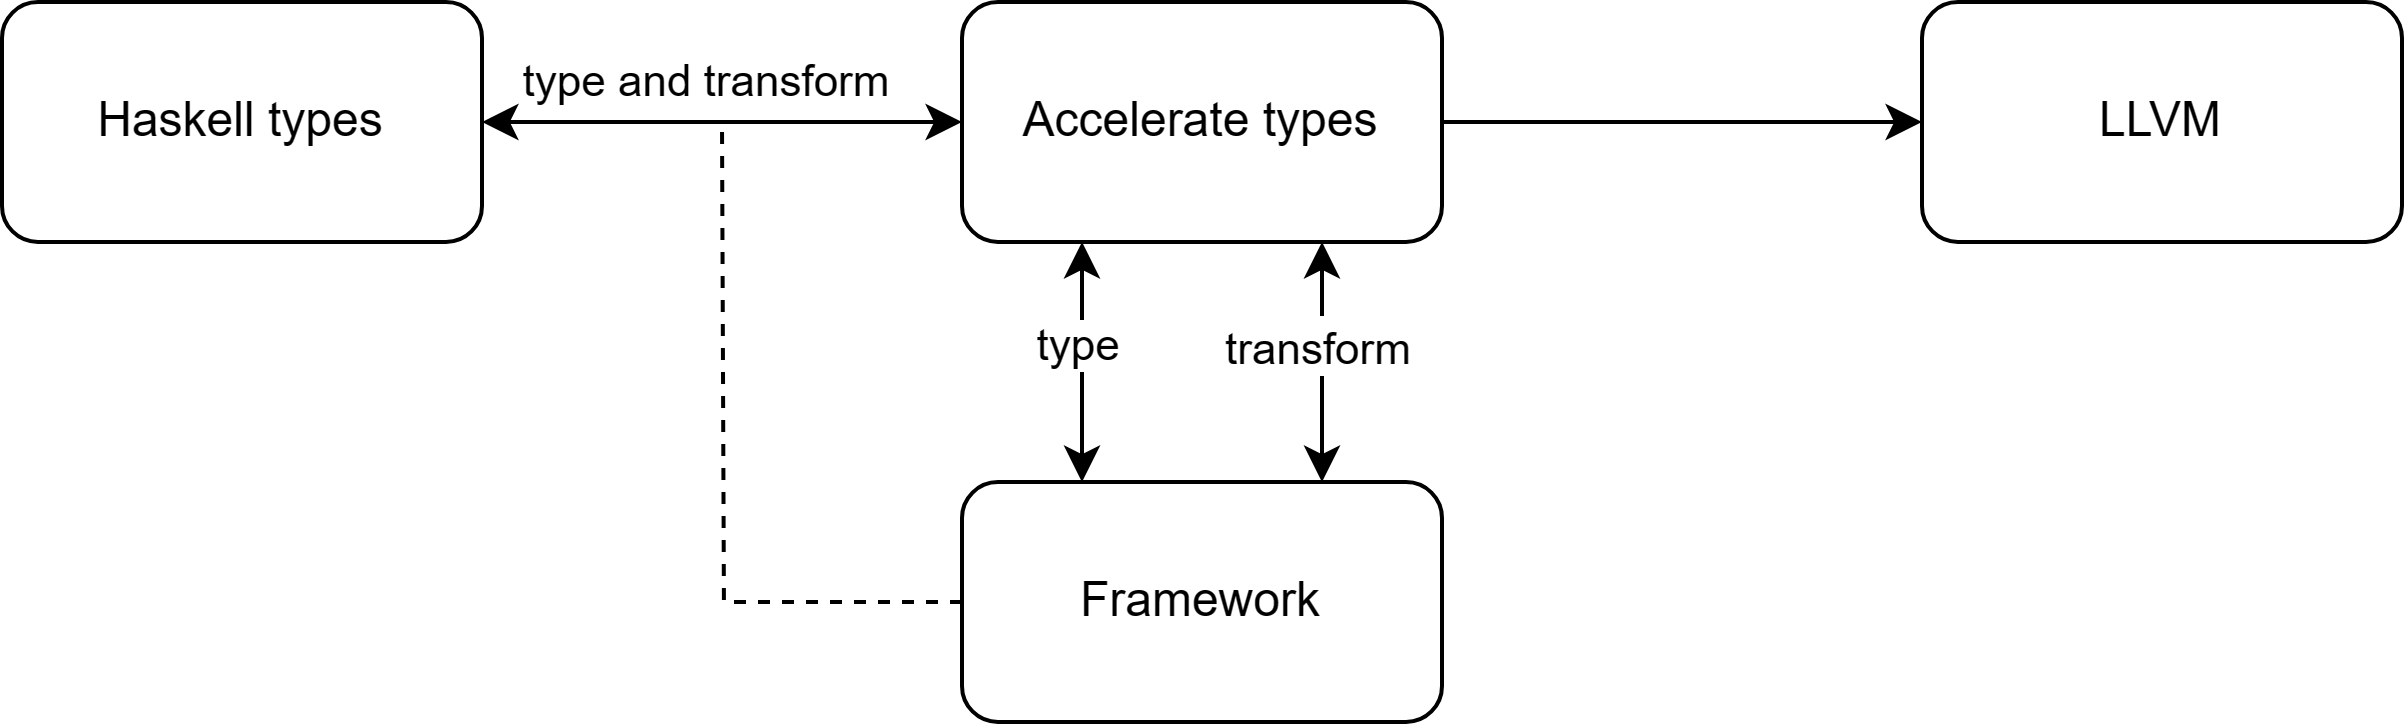
\includegraphics[scale=0.15]{framework.png}
\end{figure}

\newpage

\subsubsection{Framework}

The composition of types is enforced through a GADT, as stated within the type-level programming section.
As such a type can only have three cases; the empty type \type{()}, the primitive type \type{a} and the composed type \type{(a, b)}.
An initial attempt would be to traverse the structure and apply a function to each primitive type.
This means we need a function that discriminates between primitives types at the value level.
This is possible in most embedded languages, as the abstract syntax tree itself is represented through a GADT.

\paragraph{Traversing}
A generic way to apply a function on each primitive type is hard to define.
Each pattern match will refine the type further, which means we need a function that operates on multiple types.
When passing a polymorphic function to a higher-order function it is not instantiated on the refined type, which means we cannot apply it.
A solution is to explicitly limit the scope of type variables, such that it is local to each recursive call.

\begin{verbatim}
    traverse :: Monoid r => (forall v. Type v -> r) -> Structure e -> r
\end{verbatim}

A generic traversal of a structure is extremely powerful and the first step to a datatype-generic implementation.
The next step is traversing over the values of a structure, which is only a small step up.
It simply includes an expression with the same type as the structure, which is also refined when pattern matching on the structure.
This allows for functions to operate on fields within the datatype individually, but is restrictive in that it does not account for the hierarchy it exists in.
A more involved traverse function makes available how a primitive type can be inserted and retrieved from the structure. 

\begin{verbatim}
    type Insert value expression   = value -> expression -> expression
    type Retrieve value expression = expression -> value 

    traverse :: Monoid r => Structure a 
                         -> (forall v. Type v -> Insert v e -> Retrieve v e -> r) 
                         -> Insert a e 
                         -> Retrieve a e 
                         -> r                  
\end{verbatim}

The \type{Retrieve} function recursively accumulates the further we traverse into the structure.
The \type{Insert} function is slightly more involved, as it is recursive on the composed value.
Normally this would just be the input expression, but we are operating on the structure and do not have access to the actual expression.
Fortunately the \type{Retrieve} function is available to construct the expression to that point, which make the traversal function quite simple and compact.

\newpage

\paragraph{Intermediate}

The traversal function is the foundation for operating on two structures, required to construct and deconstruct variant types.
It is possible to create a mapping by traversing the other structure for each primitive value.
This is both redundant and highly complex when removing values from the available mappings.
The intermediate representation of a list, also used for computing the type representation, only requires a single traversal for each structure.
This requires an heterogeneous list with all the different primitive types.
Extensional types allow a type variable to be hidden, and thus they can be stored in a singe list.

\begin{verbatim}
    data Field e = forall v. Field (Type v) (Insert v e) (Retrieve v e)

    fields :: Structure e -> [Field e]
    fields = traverse (\type insert retrieve -> [Field type insert retrieve])
\end{verbatim}

Normally extensional types results in functions not being able to discriminate between the hidden types.
As the primitive types exist within a GADT, pattern matching on \type{Type v} will reveal the type to the type system.
A structure can now be constructed or destructed by folding over such a list, but more importantly the fields can be compared between structures.

\paragraph{Isomorphism}

An undiscussed constraint is that the \type{construct} and \type{destruct} functions must be isomorphic from each other.
Both must map primitive types to the same fields, otherwise we cannot retrieve the same type from the representation.
A simple way to achieve this is by creating both within the same function, such that all mapping decisions are inherently isomorphic.
This is trivial with access to the \type{Field} type, as we have access to functions that insert and retrieve the value.

\begin{verbatim}
    decisions :: forall v t. (Elt v, Elt t) => (Exp v -> Exp t, Exp t -> Exp v) 
    decisions = ...

    construct :: forall v t. (Elt v, Elt t) => Exp v -> Exp t
    construct = fst (decisions @v @t)

    destruct :: forall v t. (Elt v, Elt t) => Exp t -> Exp v
    destruct = snd (decisions @v @t)
\end{verbatim}

It does mean that the constructor \type{v -> t} might make different decisions than the constructor \type{t -> v}, as decisions are made based from the perspective of one side. 
This is not a problem as constructed types must always be destructed first.
The \type{t} type within the \type{decisions} function is allowed to have spare fields, as they are the undefined fields within an union.

\paragraph{Steps}

To avoid a local optimum in the representation several iterations must be done within the \type{decisions} function.
A matching function determines whether there exist a mapping between two fields, and returns the functions that transform between the two primitive types.
This makes the decision function extensible, as long as the user specifies the relation between two fields.
Matching functions can be provided in order of preference.
An implementation can in some cases be made more efficient by sorting before matching, but this reduces the generality of the function. 
Some cases might require a custom \type{decisions} function, such as inserting multiple fields into a single field.
In general the implementation should be tailored to the implementation language.

\newpage

\section{Implementation}

Currently we established a way to generate efficient representations through type-level programming.
Mapping between these representations are established generically through datatype-generic programming.
This is sufficient to represent the initial sought after abstraction around variant types.

\begin{verbatim}
    data Collection (types :: [*]) = VariantWise (Storage types) 
                                   | ElementWise [Variant Compact types]
\end{verbatim}

While the implementation is heavily tailored to Haskell, it is not unfeasible to implement such a framework natively within a language.
This chapter centres around implementation details specific to Haskell and Accelerate.
In this first section Accelerate related details are explored, while the second section discusses the implementation of previously discussed (de)constructors.
The third section recuperates on the initial performance considerations and benchmarks the different approaches on an existing raytracer.

\subsection{Accelerate}

Accelerate is a data-parallel array language deeply embedded within Haskell.
An abstract syntax tree (AST) is created and optimized by Accelerate within Haskell's runtime system.
This greatly improves useability, as it can function as an Haskell library, at the cost of executing code within another runtime system.
The garbage collection of the Haskell runtime system is speculated to hinder performance\cite{accelerate-performance}. 
A type-safe interface to the compiler infrastructure LLVM enabled the creation of two backends: GPU and multi-core CPU's\cite{accelerate-llvm}. 
These backends can be used to execute a small set of collective operators in parallel; such as \type{map}, \type{fold} and \type{stencil}. 

\begin{verbatim}
dotp :: Acc (Vector Float) -> Acc (Vector Float) -> Acc (Scalar Float)
dotp xs ys = fold (+) 0 (zipWith (*) xs ys)
\end{verbatim}

The inherit thread-safety and fixed set of collective operators guarantee a consistent application of data-level parallelization.
It in addition allows for these collective operators to be heavily optimized in isolation, but also in relation to other collective operators.
A naive implementation of \type{dotp} would create an intermediate array for the results of the \type{zipWith} function\cite{accelerate-array-fusion}.
Fusing these operations would eliminate an iteration and the intermediate array, at the cost of potential register pressure. 
Accelerate fuses these collective operations, unless the fusion introduces duplicate work or the \type{compute} function is explicitly called.  
As Accelerate is embedded within Haskell, it uses algebraic data types and tuples for composite datatypes.
Datatypes must be {\it lifted} into the abstract syntax tree of Accelerate, which is implemented for all native types.
The \type{Exp} datatype represents the embedded representation.
User-defined datatypes can also be lifted with the previously discussed \type{Elt} class.
As functions are written on the embedded representation, there is no type-safety when working with Algebraic Data Types.

\begin{verbatim}
    data Maybe a = Just a | Nothing

    instance Elt Maybe a where
        type EltR Maybe a = (TAG, a)
    
    fmap :: (Exp a -> Exp b) -> Exp (Maybe a) -> Exp (Maybe b)
    fmap f (tag, value) = ...
\end{verbatim}

The function retrieves the embedded \type{(TAG, Float)} type, not the sum type \type{MaybeFloat}.
Accelerate resolves this disconnection between surface and embedded representations through the use of {\it pattern synonyms}.

\paragraph{Pattern Synonymns}

A pattern synonym can be seen as an abstract constructor for a datatype.
While it is possible to achieve the same through regular functions, pattern synonyms also have the opportunity to act as a deconstructor.
Concretely it means pattern synonyms can been pattern matched against, which mean they act interchangeably to a normal datatype.
As pattern synonyms cannot share their name with their surface type an underscore is used to denote the difference. 
A limitation is that the compiler cannot prove the cases to be exhaustive, but completeness can be annotated with a pragma.

\begin{verbatim}
    pattern Just_ x <- (1, x)
        where Just_ x = (1, x)
    
    fmap :: (Exp a -> Exp b) -> Exp (Maybe a) -> Exp (Maybe b)
    fmap f (Just_ a) = Just_ (f a)
    fmap f Nothing_  = Nothing_
\end{verbatim}

It can be tedious to define pattern synonyms for all user defined datatypes, which is why Accelerate uses meta-programming to generate all constructors at compile-time.
Pattern synonyms can be extremely powerful and can be used to create a polymorphic constructor for structural sum types. 
Rather than a nominal constructor we use the position in the sum type, which can be statically constrained to the amount of variants.
It can even be defined through a type-level natural number, but this requires type annotation for each use.
For useability the pattern synonyms \type{Con0, Con1,...} are defined to avoid the need for explicit type annotations.

\begin{verbatim}
    pattern Con :: (Elt (IX n vs), Elt (f vs)) => Exp (IX n vs) -> Exp (V f vs)
    pattern Con v <- (matchable (toWord @n) -> Just v)
        where Con v = constructable (toWord @n) (construct v :: Exp (f vs))

    type Maybe a = Variant Compact [a, ()]

    fmap :: (Exp a -> Exp b) -> Exp (Maybe a) -> Exp (Maybe b)
    fmap f (Con0 a)  = Con0 (f a)
    fmap f (Con1 ()) = Con1 ()
\end{verbatim}

In some cases it might be preferable to have a descriptive name, which can be done by creating a new pattern such as \type{pattern Nothing = Con1 ()}.
This will work on all sum types that have \type{()} as second data constructor, which one might consider to comprise type-safety.
The type can be constrained to only work for \type{Variant Compact [a, ()]}, but there cannot be any distinction between types that are composed similarly due to structural typing.  
A solution is to explicitly define a new datatype and derive all functionality through the variant type.

\paragraph{Pattern Matching}

Accelerate is deeply embedded within Haskell, which means a program effectively constructs an abstract syntax tree at the runtime of Haskell.
Pattern matching occurs while constructing the abstract syntax tree, which means we are effectively trimming the tree rather than extending it.
Stated more generally it is not possible to represent choice elements within a deeply embedded representation through the surface representation.
Manual control flow is possible but Accelerate circumvents this restriction by explicitly defining all choice elements within a datatype.
When encountering a datatype with multiple choices, the function is repeatedly evaluated on a dummy type which contains the corresponding choice element.
Each deconstructor can therefore match only on the dummy type with the corresponding tag, which mean all possible branches can be obtained.
This is possible as \type{pattern synonyms} do not have to be isomorphic and the stub type is ignored within the Accelerate compiler.
As pattern matching cannot be overloaded in Haskell, the \type{match} operator is used to generate all choice elements recursively\cite{accelerate-pattern-matching}.

\newpage

\subsection{Result}

There are no setup requirements for using the variant type within Accelerate code.
Concretely, it is sufficient to use the \type{Variant} type constructor and the \type{Con0, Con1, Con2...} data constructors.
The expected behavior is that of a traditional sum type, where pattern matching happens on the current active variant. 
The intersect function discussed within the introduction only has to be written once, irregardless of any low level optimizations.
These optimizations include a variant type collection with multiple representations, multiple memory representations and efficient (de)-constructor of variant types.
The previously discussed \type{Primitive} and \type{Intersect} function can now be defined.

\begin{verbatim}
    type Primitive = V Compact [Sphere, Plane]

    intersect :: Exp Primitives -> Exp Pos -> Exp Dir -> Exp Distance
    intersect (Con0 sphere) = sphereIntersect sphere
    intersect (Con1 plane)  = planeIntersect plane
\end{verbatim}

\paragraph{Memory Representation}

The \type{Compact} type already deduplicates primitive types of the same size, which makes the memory representation of \type{Primitive} already quite compact.
A more aggressive approach is to deduplicate on larger fields, which requires defining a type with the same kind \type{[*] -> r}. 
Such type can be defined through pre-existing type-level functions, which can then be used as layout for all variant types.
The datatype-generic constructors adapt independently to the derived type and resort to truncation when deconstructing these fields.
As such, the \type{intersect} function does not have to adapt to a memory representation optimization.

\paragraph{(De)constructor}

The \type{Variant} type uses a single tag to represent the active variant, which is used by the \type{Case} operator to pattern match.
This is often quite performant, but in some cases it can be preferable to unconditionally execute a function.
The \type{Maybe} type can always unconditionally execute, as the \type{Nothing} constructor does not have any fields.
This is impossible with variant types that deduplicate fields, as unconditionally executing would impact the correctness.
With the datatype-generic functions a bitmask can be unconditionally generated, which masks side-effects of all unconditionally executed functions.  
Rather than integrating this within the \type{Variant} type, it can be used as replacement for the pattern matching \type{match} operator.

\paragraph{Collection}

The datatype-generic functions allow for a collection of \type{Primitives} to be completely agnostic to the representation.
For a variant-wise collection pattern matching is redundant, which means to be effective all control-flow paths of the \type{intersect} function must be extracted. 
Pattern matching will effectively occur on the Haskell side, which is trivial due to embedded pattern matching already making choice elements explicit.
Distributing the \type{intersect} function over multiple arrays, within a collection of \type{Primitives}, can therefore be done.
With this many collective operations can be supported, including ones that modify the identity of such a collection.
These collective operators are currently not implemented beyond the necessary operators to support benchmarking.

\begin{verbatim}
    example of some collection functions
\end{verbatim}


\newpage

\subsection{Benchmarks WIP}

A concrete performant way to operate on multiple variants was not an objective in its own right, due the nature of many components being able to influence the performance of an application.
In this section previously discussed optimizations are applied while preserving the type identity of the functions.
The \type{nearest} function is used as example, which computes the nearest primitive intersection of ray.
This is fused into a single traversal, which ..

\begin{verbatim}
-- | nearest primitive that intersects with a ray
nearest :: Exp Pos -> Exp Dir -> Collection [Sphere, Plane] -> Acc (Scalar Distance)
nearest position direction = fold min Miss . map (intersect position direction)
\end{verbatim}



\begin{center}
    \begin{tabular}{ | m{14em} | m{8em}| m{8em} | m{8em} | } 
      \hline
      {\bf Type} & {\bf Interpreter} & {\bf CPU} & {\bf GPU} \\ 
      \hline
      Variants         & 6.22ms & 9.54ms & 8.07ms\\ 
      \hline
      Elements         & 3.66ms & 5.50ms & 5.24ms\\ 
      \hline
      Sorted           & 3.79ms & 5.49ms & 5.28ms\\ 
      \hline
      Compact Elements & 5.09ms & 6.78ms & 6.60ms\\ 
      \hline
      Compact Sorted   & 4.97ms & 6.72ms & 6.91ms\\ 
      \hline
    \end{tabular}
\end{center}

scaling to larger size

\begin{center}
    \begin{tabular}{ | m{14em} | m{8em}| m{8em} | m{8em} | } 
      \hline
      {\bf Type} & {\bf Interpreter} & {\bf CPU} & {\bf GPU} \\ 
      \hline
      Variants         & 100.4ms & 9.66ms & 8.39ms \\ 
      \hline
      Elements         & 104.9ms & 5.45ms & 4.58ms \\ 
      \hline
      Sorted           & 101.3ms & 5.48ms & 4.89ms \\ 
      \hline
      Compact Elements & 119.4ms & 6.81ms & 6.64ms \\ 
      \hline
      Compact Sorted   & 97.90ms & 6.78ms & 6.71ms \\ 
      \hline
    \end{tabular}
\end{center}

\newpage

\section{Discussion}

In this paper some fundamental choices have been made without extensive argumentation.
This chapter is used to highlight these choices and provide further reasoning for the choices that have been made.
It also highlights some limitations of the framework and ways these can be resolved.

\subsection{Benchmarks WIP}



\subsection{Embedded Domain-Specific Language}

Libraries and domain-specific languages that are embedded construct their user-defined-types through the host-language.
A shallow embedding operates directly on types native to the host-language, while deep embeddings construct an abstract syntax tree that is later evaluated.
The latter offers flexibility on how user-defined types are implemented, as types exist both on the surface level and as construct within the abstract syntax tree.   
There are several approaches, which have been subject to research in the domain of circuit design.

\begin{itemize}
    \setlength\itemsep{0em}
    \item {C$\lambda$aSH} is not deeply embedded and operates on user-defined types through generics\cite{clash}. 
    \item Hydra has the deep embedding constructs nested into the shallow embedding constructs\cite{hydra}.
    \item Kansas Lava has both embeddings exist in parallel under an encasing type\cite{kansas-lava}.
    \item ForSyDe has both embeddings exist separately as standalone types\cite{forsyde}.
\end{itemize}

An observation is that user extendability is limited on deeply embedded constructs as execution models must be updated.
A proposed approach is to have a small deeply embedded core language that only supports constructs that are relevant for combinatorial optimizations\cite{shallow-and-deep}. 
The shallow embedding can be used to create an extensible and user-friendly interface to this core language.
In the context of data-parallel applications and variants this leans itself to an implementation in the host-language.
This distinction is irrelevant for languages that are not embedded in other languages.

\subsection{Datatype-generic programming in Haskell}

Current Accelerate derives the \type{Elt} class generically through Haskell's native datatype-generic framework.
It traverses the structure of the datatype, for each layer providing both the type and the transformation.
As these are intrinsically linked, deduplication must be represented both on the value-level and type-level.
The {\it Recursive Tagged Union}\cite{accelerate-sum-types} uses this approach, which proved to be problematic and complex.
One concern was that replacing the \type{Elt} class was considered to be a too invasive of an operation\cite{accelerate-sum-types}.
This means the \type{Elt} class must be derived from the implementation class, which limits user extendability. 
It is also not possible to sort the types on the type-level, as closed type families do not have an intrinsic link to its value-level construct.
An implementation that is fully modular and extendible on both the value-level and type-level prevent these complications.
Explicit derivation of the \type{Elt} class is also not required, as the sum type itself is effectively a polymorphic datatype that implements the \type{Elt} class. 

\subsection{Limitations}

\paragraph{Surface type}

As structural sum types do not exist in Haskell, it is not apparent what the corresponding surface type should be.
Currently there exists no mapping from the variant type to a surface type, which might sound more problematic then it really is.
It means (de)-constructing the variants must be done in the Accelerate code, rather than Haskell.
A solution can also be to just use a dynamic type, or make a direct mapping to an existing open sum library.

\paragraph{Nested pattern matching}

Since tags are statically determined for each type individually, nested pattern matching is not trivial. 
Currently the datatype \type{TagR} is used, where \type{Just (Just a)} is represented as \type{TagRtag 1 (TagRtag 1 (TagRsingle a))}. 
Pattern matching on the first \type{Just} would remove one layer, and the rest is propagated along.

\begin{verbatim}
    data TagR a where
        TagRtag    :: TAG -> TagR a -> TagR (TAG, a)
        TagRunit   :: TagR ()
        TagRsingle :: ScalarType a -> TagR a
        TagRpair   :: TagR a -> TagR b -> TagR (a, b)
\end{verbatim}

An important detail is that these tags are generated statically, for all possible permutations.
In a type with deduplicated fields the {\it nested} datatype is not necessarily available, as it might be constructed through different fields.
As the \type{TagR} is constrained to the same structure as the encapsulating type, it is not possible to list all possible permutations through the \type{TagR} type.
A solution is to just lose the type-safety on the \type{TagR} type, and allow for more flexibility.
As the \type{TagR} type is integrated with the \type{Elt} class, a change would require a lot of code changes within Accelerate.

\paragraph{Unified tag}

An extension of the previous discussion is the use of a single tag, for multiple nested tags.
It involves operations to extract and construct the tag, which can be computationally expensive.
Currently the deduplication algorithm has no knowledge of tags at all, and sees them as any other field.
An implementation would complicate both the deduplication process and automatic derivation of (de)-constructors.
A temporary solution would involve simply flattening the sum type, which would also be more performant in the general case.
Another solution would be to change perspective and argue tags are datatypes with a statically determined size depending on the amount of choices they represent.
Both the type-level and datatype-generic part would handle tags as any other fields, and can upscale them to an existing datatype.

\paragraph{Struct}

While it possible to derive struct-like memory representations, Accelerate does not (yet) have the instructions to insert and extract those values.
As primitive types are implicitly distributed over multiple arrays, there is no need to operate on a type within a larger type. 
It in addition does not allow types existing outside the predefined types, which means memory representation is limited to that set of types.
A solution would be to add an (untyped) type with a variable size and corresponding instructions to extract (aligned) data.

\newpage

\section{Conclusion WIP}

\subsection{Future Work}

\newpage

\bibliographystyle{plain}
\bibliography{refs}

\end{document}